%!TEX TS-program = xelatex
%!TEX encoding = UTF-8 Unicode

% Load Thesis Class
\documentclass{DEIThesis}

\title{Simulation Study, Design and Implementation of 5G NR Layer-2 Protocols for Non-Terrestrial Networks}

\author{Francesco Rossato}
\studentId{2082121}

% Advisor
\advisor{Professor Michele Zorzi}

% If you are co-advised
\coadvisor{Professor\ Marco Giordani}
\coadvisorsUniversity{University of Padova}
\cocoadvisor{Dr. Matteo Pagin}
\cocoadvisorsUniversity{University of Padova}

\university{University of Padova}
\mastername{ICT for Internet and Multimedia}
\graduationDate{03-09-2024}
\academicYear{2023/2024}

\begin{filecontents*}[overwrite]{\jobname.xmpdata}
    \Title{Simulation Study, Design and Implementation of 5G NR Layer-2 Protocols for Non-Terrestrial Networks}
    \Author{Francesco Rossato}
    \Language{en-EN}
    \Keywords{ntn\sep 5G\sep non terrestrial networks \sep francesco rossato\sep HARQ\sep scheduler\sep layer 2}
\end{filecontents*}

% Document

\begin{document}
    % The front matter (Cover, ToC, Abstract, etc...)
    \frontmatter

    % The main content
    \mainmatter
    %!TEX root = ../main.tex

\chapter{Introduction}
\label{chp:intro}

The term \ac{NTNs} denotes a category of networks where at least one link is routed via an aerial or space-borne vehicle such as \ac{HAPs}, \ac{UAVs} or telecommunication satellites.

\section{The focus on non-terrestrial networks}
The Third Generation Partnership Project \footnote{\href{https://www.3gpp.org}{\texttt{3gpp.org}}} (3GPP), the standardization body developing protocols for mobile communication networks, recently put a great emphasis on the importance of the integration of different access technologies along with the existing terrestrial mobile telecommunication infrastructure \cite{3gpp-tr-21.917}.

The envisioned future for mobile communications, starting with the already established 5G \ac{NR} and expanding with the new sixth-generation cellular networks (6G), foresees the integration of a non-terrestrial component. The latest \ac{3GPP} releases (Rel. 17 and Rel. 18) require 5G and 6G networks to be able to provide non-terrestrial satellite access complementing the already existing terrestrial access technologies \cite{overview-rel-17-18-saad} \cite{5g-nr-communication-geo-leo-maattanen}.

\section{Limitations of terrestrial networks}
The following paragraphs present a few scenarios where terrestrial networks have some limitations, and \ac{NTNs} can be used to provide connectivity.

\subsection{Remote places}
While \ac{TN} make the well-established foundation of today’s mobile communication infrastructure, their own nature poses some intrinsic limitations to their deployment in certain scenarios, especially in rural and remote areas. Conditions such as harsh terrain and geographical impediments act as natural barriers to the deployment of terrestrial infrastructure. Moreover, ground infrastructure requires the presence of an already established reliable power grid, driving up the costs that telecommunication companies would have to sustain.
The population density is often low in remote and rural places, so the already high infrastructure cost will hardly pay for itself, making this kind of market even more unattractive to private investors and further limiting the possibility for the people living there to access a resource which is becoming increasingly more important.

As studied and documented in \cite{6g-challenge-opportunity-base-pyramid}, the issue of an inadequate broadband coverage in rural regions is an enormous challenge, but also a great opportunity to kick-start the economy of currently underdeveloped countries, promoting a more fair access to the internet and alleviating the problem of digital divide between different parts of the world.

\subsection{Redundancy}
Another limitation of the current terrestrial infrastructure is the lack of redundancy and robustness against natural disasters. Extreme events such as earthquakes, fires and floods, but also deliberate behaviors such as targeted attacks by terrorist organizations and sabotages can disrupt the connectivity even for a long period of time, causing significant economical damage and hindering the already difficult rescue efforts, potentially leading to loss of lives.

The simple installation of a greater number of base stations is not a viable solution because they all share the same weaknesses.

In this scenario, \ac{NTNs} can act as redundant access methodology to decrease downtimes of terrestrial infrastructure, provide emergency communication services and also additional capacity when required. 

\subsection{Long distances and sensors}
Remote equipment, offshore plants and distribution grids will also benefit from the research carried out in this field, since providing terrestrial connectivity in those scenarios is a challenging task. The installation of an underwater optical fiber link to serve a single endpoint, such as an offshore power plant in the ocean, would bear a disproportional cost compared to the functions required, and maintenance would be another challenging and expensive task. 
The deployment of a non-terrestrial network would provide connectivity on a global scale, therefore allowing internet access in isolated places without the need for a dedicated connection.

Consider now the problem of connecting of a number of sensors placed in a large area. When distances are large, solutions may either be the densification of radio stations or the use of a lower frequency in order to have a less severe propagation loss. However, those approaches have their downsides and are not always feasible. In this case, the large coverage area of \ac{NTNs} will undoubtedly be useful to provide internet connection \cite{performance-ntn-support-iot-wang}.

\paragraph{} Other scenarios where \ac{NTNs} can become useful in overcoming the limitation of their terrestrial counterpart are well described in \cite{ntn-6g-era-challenges-giordani} and \cite{potential-multilayered-nierarchical-ntn-wang}.

\section{Satellite types}
Satellites are divided in three different categories depending on their orbiting altitude: \ac{GEO}, \ac{MEO} \ac{LEO} satellites. Each one has its own characteristics, as briefly described below.

\subsection{GEO satellites}
orbiting at 35.786Km, \ac{GEO} satellites appear stationary since their orbiting period is the same as the Earth rotation period. This vastly simplifies the tracking for the ground equipment, since once the position of the \ac{UE} is known, the relative position of the satellite is known, too.
    
Since \ac{GEO} satellites are geostationary, continuous coverage to a designated area can be provided using as little as a single satellite, while the use of non-\ac{GEO} satellites would require the deployment of a constellation, which is both more complex and more expensive.

Their higher altitude creates a large cell footprint, larger than both \ac{MEO} and \ac{LEO}, so the overall cost to provide coverage to the same area is lower.

The disadvantages of \ac{GEO} satellites are mainly linked to the large distance with the \ac{UE}: the transmission power and the antenna gain have to be higher to account for the greater propagation losses, and the propagation delay of the signal travelling at the speed of light is about 120ms, so if the \ac{UE} sends a request to a server at time zero through a \ac{GEO} link, the best-case delay will be of half a second without considering any protocol-related delay.

In addition to the positive aspects previously discussed, the larger cell footprint also means that a single satellite will be serving a massive number of users, so the total available capacity will have to be shared between a bigger number of actors, and the throughput experienced by each one of them will be reduced. 
Moreover, the high number of users leads to a large rate of initial access  requests, with the possibility of channel saturation as described in \cite{3gpp-tr-38.811}.

\subsection{LEO satellites}
Orbiting below the altitude of 2.000Km, \ac{LEO} satellites are the most promising solution in the realm of \ac{NTNs} for a number of reasons hereby discussed.
    
The lower altitude entails a shorter propagation delay, and the smaller coverage area of each satellite means that the total number of users that need to be served is smaller. 

The cost per satellite is significantly smaller than \ac{GEO} and \ac{MEO} satellites. However, given that they are not geostationary, a large constellation is needed to provide a continuous service, driving up the deployment costs significantly. As an example of those constellations, Fig. \ref{fig:starlink_constellation} depicts the \ac{LEO} satellites employed by Starlink\footnote{Starlink is a satellite internet constellation operated by Starlink Services, LLC, a wholly-owned subsidiary of American aerospace company SpaceX.}, with 4.808 units in service at the time of writing\footnote{Source: \href{https://satellitemap.space/}{\texttt{satellitemap.space}}}.

\begin{figure}[ht]
    \centering
    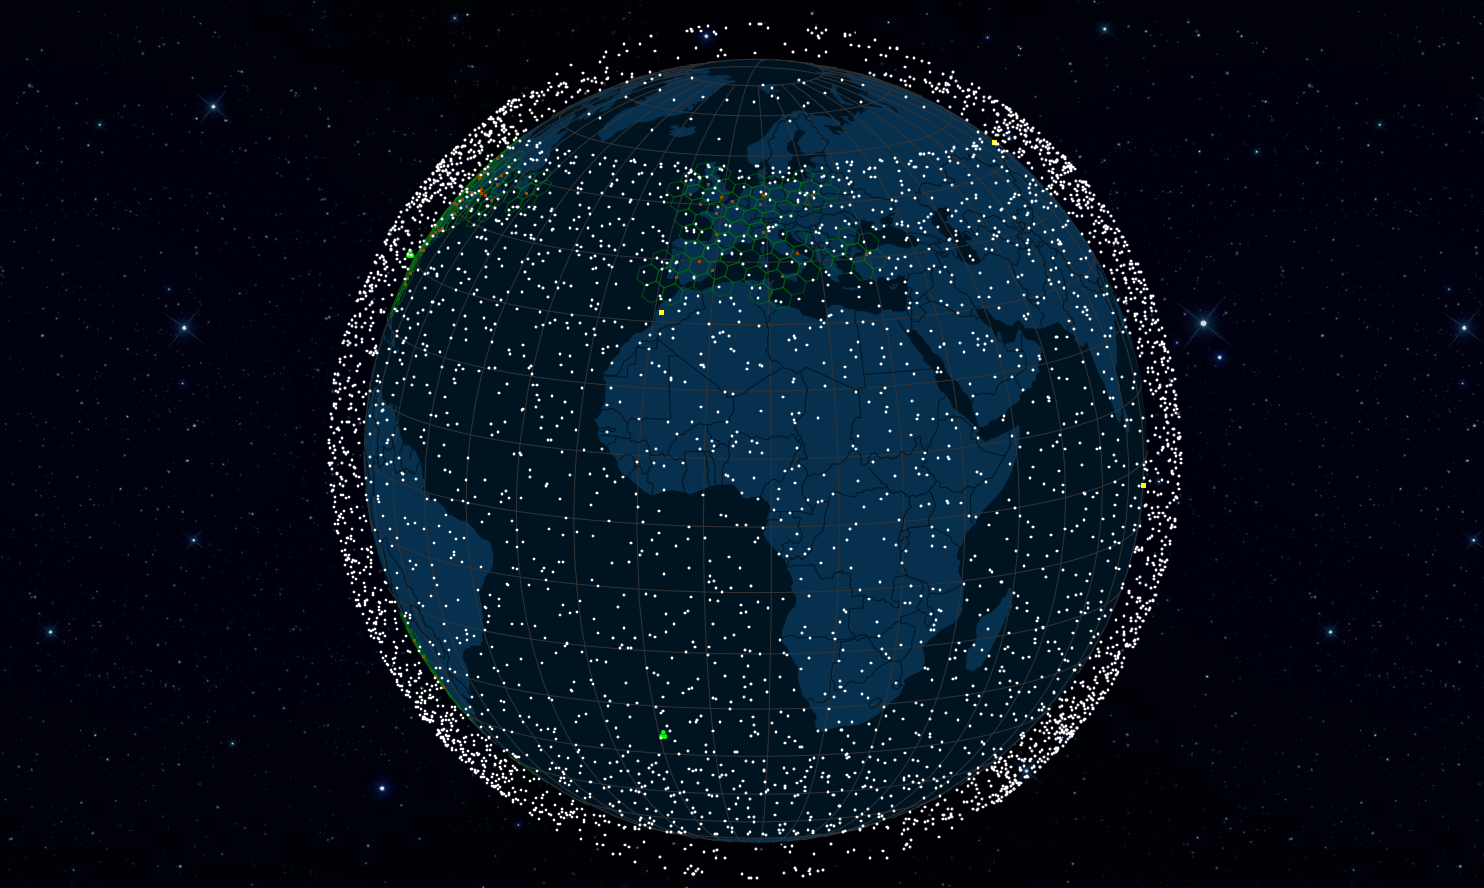
\includegraphics[width=0.7\textwidth]{res/starlink-constellation.png}
    \caption{Starlink constellation as July 2024. Source: \href{https://satellitemap.space/}{\texttt{satellitemap.space}}}
    \label{fig:starlink_constellation}
\end{figure}

The smaller altitude at which \ac{LEO} satellites orbit enables the use of higher frequency bands, since the experienced path loss is smaller compared to \ac{GEO} satellites. This in turn allows for higher throughput, as detailed in \cite{satellite-communication-mmwave-giordani}

The aforementioned solutions are not to be considered mutually exclusive. In fact, the multitude of possibilities that their combinations offer open to the study of various different scenarios, as detailed in \cite{potential-multilayered-nierarchical-ntn-wang}

\subsection{Current solutions}
Current solutions for non-terrestrial communication do exist, but they mostly rely on telecommunications satellites placed in the \ac{GEO}, at a height of 35.786 km. The distance that the signal has to travel offering limited throughput and large delays. While \ac{LEO} constellations (400 km to 2.000 km) have proven to be a valid alternative, providing higher throughput and lower latency \cite{main-features-5g-nr-ntn-yun}, they have the drawback of an increased Doppler shift due to their high speed relative to ground \cite{satellite-communication-mmwave-giordani}, and there is still no international standard with regard to the communication protocols to use. 

\paragraph{}
This scenario led \ac{3GPP} to identify some work to be done to integrate \ac{NTN} in cellular standards, calling for long-term research in this field \cite{satellite-communication-mmwave-giordani}. This work will mainly focus on the 

\paragraph{}\todo{move this to state of the art} Focusing on the \ac{MAC} sublayer, the large propagation delay of satellite links affects different aspects, making the actual implementation not suited for a \ac{NTN} scenario. In the \ac{HARQ} protocol, the retransmission timeout is likely to expire before a single \ac{RTT}, leading to unnecessary retransmissions. Moreover, the limit on the maximum number of concurrent \ac{HARQ} processes leads to a stop-and-wait behaviour, which may increase the energy consumption \cite{3gpp-tr-38.811}. On the other hand, it has been noted that disabling \ac{HARQ} would lead to an even worse performance penalty, therefore requiring a redesign for \ac{NTN} \cite{5g-beyond-5g-ntn-trends-vanellicoralli}. Another 5G \ac{NR} protocol which is negatively impacted in \ac{NTN} is the initial access, since users at the center of the cell face a smaller propagation delay with respect to users at the cell edge \cite{5g-beyond-5g-ntn-trends-vanellicoralli} \cite{applying-nr-technologies-in-ntn-lee}. As a result, preambles of \ac{UE}s placed near the cell edge may reach the satellite when the \ac{RACH} opportunity has already expired, which may lead to collisions. During the initial access phase, \ac{UE}s are not aware of their propagation delay, and the high mobility of \ac{gNB}s on \ac{LEO} satellites causes a non-negligible Doppler shift. Those factors vary with the relative position and speed between the \ac{UE} and the \ac{gNB}, and the protocols for initial access must be modified in \ac{NTN} to account for them \cite{ntn-from-5g-6g-hassan}. 
\paragraph{}
It is clear that the future of mobile networks envisioned by \ac{3GPP} embraces \ac{NTN}s, and considerable work has to be done. Research will bear a high impact towards a more connected, equal opportunity world. 

\section{Currrent state of the art}
\todo{types of payloads: regenerative, and transparent or bent pipe}
    %!TEX root = ../main.tex

\chapter{Non-terrestrial networks}
\label{chp:ntn}
This chapter describes the main charateristics of \ac{NTN}s, i.e., networks where at least one link endpoint is either an aerial or space platform. Specifically, the remainder of this chapter highlights the differences between types of satellites, their advantages and disadvantages as well as the possible choices for payload types. This thesis focuses on the implementation of 5G \ac{NR} in a non-terrestrial scenario, therefore \ac{NR} terminology is used.

\section{Satellite types}
\label{sec:satellite-types}
Satellites are divided in three main different categories, depending on their orbiting altitude: \ac{GEO}, \ac{MEO}, and \ac{LEO} satellites. Each category exhibits has its own characteristics, presenting some upsides and downsides as described in the remainder of this section. Fig. \ref{fig:satellite_coverages} illustrates the different orbiting altitudes as well as estimates of the corresponding coverage areas.

\begin{figure}[ht]
    \centering
    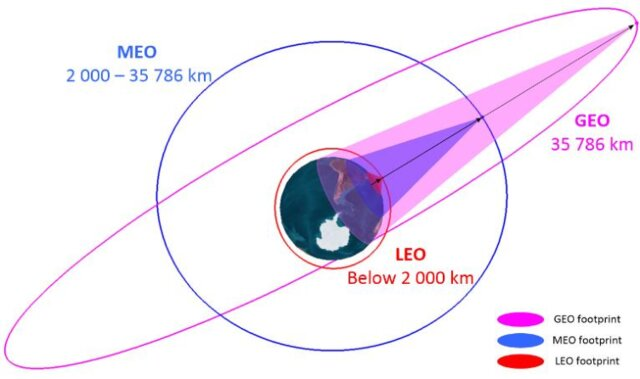
\includegraphics[width=0.9\textwidth]{res/satellite-coverages.jpg}
    \caption{Altitude and approximate coverage areas for satellites at different orbits \cite{sustainable-sat-com-6g}}
    \label{fig:satellite_coverages}
\end{figure}

\subsection{GEO satellites}
Orbiting at an altitude of 35.786Km, to an observer placed on the Earth surface \ac{GEO} satellites appear stationary, since their orbiting period is the same as the Earth rotational period.

\paragraph{Advantages}    
Since \ac{GEO} satellites are geostationary, continuous coverage to a designated area can be provided using as little as a single satellite, while the use of non-\ac{GEO} satellites requires, in general, the deployment of a constellation which is both more complex and more expensive. 

Geostationary satellites also vastly simplify the problem of the ground equipment having to be able to track the satellite. Since the satellite position is always known, once the position of the \ac{UE} is established, the relative position of the satellite can be easily estimated.

As shown in Fig. \ref{fig:satellite_coverages}, the high altitude of \ac{GEO} satellites creates a large cell footprint. Overall, while the deployment cost of a single \ac{GEO} satellite is higher than both \ac{MEO} and \ac{LEO} ones, the cost per coverage area is lower, and an almost full coverage of the terrestrial globe can be achieved using as little as three equally spaced satellites \cite{types-of-orbits-esa}.

\paragraph{Disadvantages}
The disadvantages of \ac{GEO} satellites are mainly caused by their large distance with respect to \ac{UE}s placed on the Earth surface: the transmission power and the antenna gain have to be high enough to overcome the greater propagation losses. Moreover, the propagation delay of the signal increases the baseline latency by approximately 120ms. This means that if the \ac{UE} sends a request to a server at $t=0$ through a \ac{GEO} link, the packet will be received by the destination node at least $t=240$ms. The response will then finally reach the \ac{UE} after at least $480$ms since the initial transmission. These calculations do not factor in any delay related to medium access requests, packet transmission times and processing delays, which would further increase the overall latency.

In addition to the positive aspects previously discussed, the large cell footprint also brings some downsides with it. Due to the vast coverage area, a single satellite will be required to serve a massive number of users. As a consequence, the total available capacity will have to be shared between a bigger number of equipments, and the throughput experienced by each of them will be reduced. Preliminary solutions to overcome this issue comprise, for instance, the use of beamforming to divide the covered area in smaller cells, and the employment of higher frequency bands towards Ku, K and Ka as depicted in Fig. \ref{fig:satellite-bands} \cite{advances-comm-sat-sys}.
Moreover, the high number of users also leads to a large rate of initial access requests, with the possibility of channel saturation as described in \cite{3gpp-tr-38.811}.

\begin{figure}[ht]
    \centering
    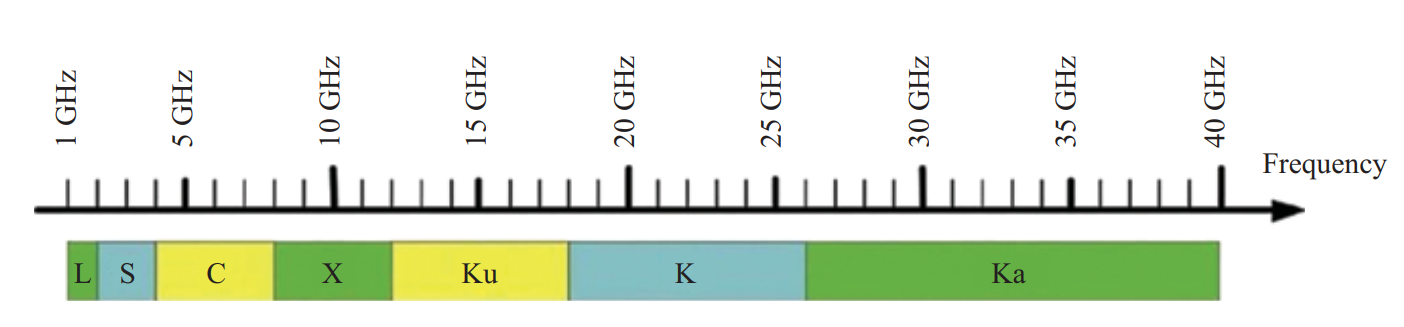
\includegraphics[width=0.9\textwidth]{res/satellite-bands.png}
    \caption{Satellite spectrum bands allocation \cite{advances-comm-sat-sys}}
    \label{fig:satellite-bands}
\end{figure}

\subsection{MEO satellites}
\ac{MEO} orbits sit between the LEO and GEO counterparts. Accordingly, all satellites orbiting between 2000 Km and 35.786 Km are considered as \ac{MEO}. This vast orbital space is mainly used by navigation systems such as GALILEO \cite{types-of-orbits-esa}.

While the propagation delay can vary a lot depending on the altitude, in general it is larger than that of \ac{LEO} and smaller than that of \ac{GEO}. The same point can be made regarding the cell size and number of served users. 

Similarly to \ac{LEO} satellites, \ac{MEO} ones do require a constellation in order to provide continuous coverage over a designated area, since they are not geostationary. Nevertheless, the number of satellites needed for providing continuous coverage is smaller than that required when using \ac{LEO} satellites, since the former can serve a larger area.


Their many downsides in addition to the lack of any substantial benefit over their competitors besides for the need for a smaller constellation makes them less than ideal candidates for applications in \ac{NTN}s.

\subsection{LEO satellites}
\label{sec:leo}
Orbiting below the threshold altitude of 2.000Km, \ac{LEO} satellites represent the most promising solution in the realm of \ac{NTNs}, mainly because they can offer really compelling throughput and propagation delay. However, the latter come at the cost of numerous disadvantages which are peculiar to satellites deployed at this altitude.

\paragraph{Advantages}
The low altitude entails a shorter propagation delay, between 2 and 6 ms. Furthermore, the smaller coverage area of each satellite with respect to \ac{MEO} and \ac{GEO} means that the total number of users that need to be served is smaller. This also enables the use of high frequency bands and the constraints of high antenna gains are less stringent compared to \ac{GEO} satellites, since the experienced path loss is much smaller. In turn, this leads to a higher throughput, more suited to satisfy the requirements of modern days broadband connectivity, as detailed in \cite{satellite-communication-mmwave-giordani}.

The cost per deployed satellite is significantly smaller than that of \ac{GEO} and \ac{MEO} satellites, and multiple deployments within a single launch are possible, further reducing the deployment costs.

\begin{figure}[ht]
    \centering
    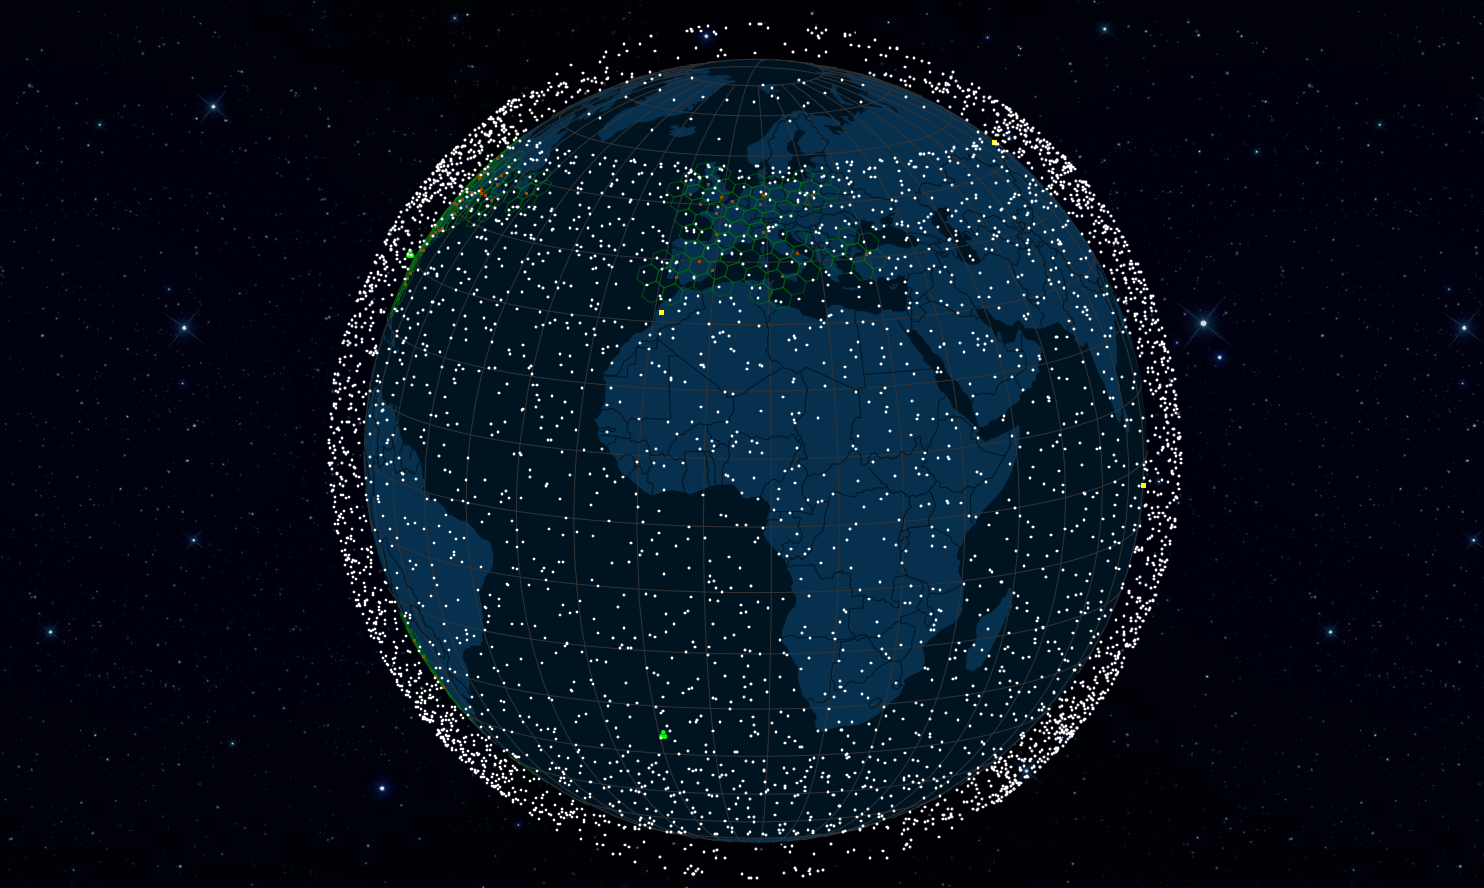
\includegraphics[width=0.9\textwidth]{res/starlink-constellation.png}
    \caption{Starlink constellation as of July 2024. Source: \href{https://satellitemap.space/}{\texttt{satellitemap.space}}}
    \label{fig:starlink_constellation}
\end{figure}

\paragraph{Disadvantages}
Given that \ac{LEO} satellites are not geostationary, a large constellation is needed to provide continuous service, driving the deployment costs significantly up. As an example of how vast those constellations can become, Fig. \ref{fig:starlink_constellation} depicts the \ac{LEO} satellites employed by Starlink\footnote{Starlink is a satellite internet constellation operated by Starlink Services, LLC, a wholly-owned subsidiary of American aerospace company SpaceX.}, counting about 4.808 units in service at the time of writing\footnote{Source: \href{https://satellitemap.space/}{\texttt{satellitemap.space}}}.


Since low orbiting satellites remain view of the \ac{UE}s only for a short period of time, with an average in-view duration of just 13 minutes as calculated in \cite{regional-coverage-analysis-leo}, all the connected users are expected to be handed over to the next available satellite within this time window. Such behavior would create a noticeable protocol overhead, consuming available channel capacity and potentially adding more latency. However, the predictable nature of this phenomenon might allow for a partial automation without requiring explicit control messages to be exchanged.

The small coverage area means that more terrestrial gateways have to be deployed, since each satellite can only communicate with the ground via the terrestrial gateways that fall within its view. A different solution to the densification of gateways is the use of \ac{ISL}, i.e., high-bandwidth links between different satellites of the constellation. The latter are used to connect satellites that do not have gateways in sight to ones that are connected to a gateway, allowing traffic to be routed to the ground via additional hops. Inter-satellite links have also to be implemented if coverage over the oceans is required. Ultimately, this further increases the high constellation deployment costs.

An additional downside affecting all the non-geostationary satellites involves their speed relative to the user equipment located on the ground. A \ac{LEO} satellite moves with a speed of approximately 7.8 km/s \cite{leo-definition-theory-facts}, thus exhibiting a non-negligible Doppler shift. This has to be compensated for, and preliminary solutions in this sense can only be applied to \ac{UE}s which feature GNSS capabilities, which is not always a reasonable assumption \cite{satellite-communication-mmwave-giordani, 3gpp-tr-38.821}. Moreover, the dependency of the network on a third-party service in order to operate properly adds a point of failure which is outside the control of the network operators. Indeed, a disruption in GPS service would halt the network capabilities.

\paragraph{}
The aforementioned advantages make \ac{LEO} satellites the most promising choice in the field of \ac{NTN}s.

\subsection{Multilayered networks}
The aforementioned orbits are not to be considered mutually exclusive. In fact, the multitude of possibilities that their combinations offer opens to the possibility of various different scenario in which the space, air, and ground layers are orchestrated to improve quality of service. An example of such multi-layer network is depicted in Fig. \ref{fig:multilayered-ntn}, showcasing a highly sophisticated non-terrestrial multilayered network scenario where different access technologies are used.

\begin{figure}[ht]
    \centering
    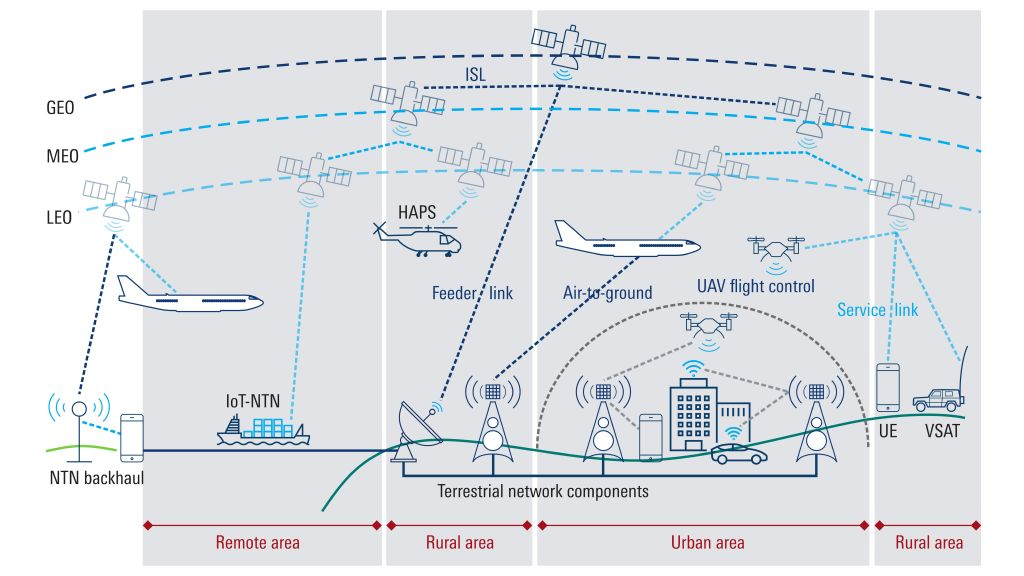
\includegraphics[width=0.9\textwidth]{res/multilayered-ntn.jpg}
    \caption{Complex multilayered \ac{NTN} scenario \cite{connecting-ntn-rohde-schwarz}}
    \label{fig:multilayered-ntn}
\end{figure}

For instance, \cite{potential-multilayered-nierarchical-ntn-wang} argues that that the use of \acp{HAP} as relays between the ground segment of the network and the upper \ac{GEO} satellite links can deliver up to six times the capacity, and better overall outage probability, than point-to-point \ac{GEO} transmissions.


\section{Types of payloads}
When implementing a \ac{NTN}, an important choice to be made is the type of payload to use. There are two main categories: bent-pipe payload and on-board \ac{gNB}. Each one has its own benefits as briefly described below.

\subsection{Bent-pipe payload}
\label{sec:bent-pipe-payload}
This is the simplest approach, where the role of the satellite consists only of  repeating the signal received from the \ac{UE} on the ground towards the terrestrial gateway. Configurations such as the one depicted in Fig. \ref{fig:ntn-bent-pipe} go by the name of bent pipe payloads and are characterized by the presence of a terrestrial g-NodeB, while the satellite has the sole purpose of providing a transparent link to the \ac{UE}.

While such solutions are by far the simplest in terms of payload complexity, the main drawback is the even longer experienced latency. Since communications between users served by the same satellite would also have to be routed through the terrestrial gateway, the overall latency increases by at least two times the propagation delay.
This solution also poses strict bandwidth requirements on the feeder link, since all the traffic must necessarily pass through it.
More complex solutions are able to route at least part of the inbound traffic autonomously, without routing everything back to earth.

\begin{figure}[ht]
    \centering
    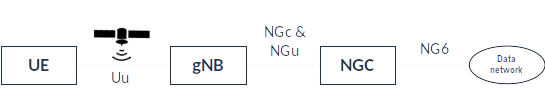
\includegraphics[width=0.9\textwidth]{res/ntn-bent-pipe.png}
    \caption{5G NR NTN architecture for access network based on satellites with bent pipe payload \cite{3gpp-tr-38.811}}
    \label{fig:ntn-bent-pipe}
\end{figure}

\subsection{On-board g-NodeB}
\label{sec:onboard-gnb}
A slightly more sophisticated approach foresees the installation of g-NodeB capabilities directly onto the satellite payload, as depicted in Figure \ref{fig:ntn-gnb-onboard}. This has the benefit of reducing the experienced latency, as well as reducing the utilization of the feeder link. Certain protocols, designed to terminate at the \ac{gNB}, can in this case reach their designated endpoint without necessitating to be routed back to the ground gateway.

\begin{figure}[ht]
    \centering
    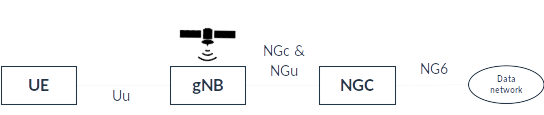
\includegraphics[width=0.9\textwidth]{res/ntn-regen.png}
    \caption{5G NR NTN architecture for access network based on satellites with on-board gNB payload \cite{3gpp-tr-38.811}}
    \label{fig:ntn-gnb-onboard}
\end{figure}

\section{Commercial solutions}
\paragraph{Legacy solutions}
Commercial solutions, initially concerning satellite-based phone calls and successively evolved to provide Internet access, have been available dating back to 2003, when the first Internet satellite was launched \cite{first_internet_sat}. However, the majority of this legacy infrastructure makes use of \ac{GEO} satellites, therefore presenting all the limitations discussed in section \ref{sec:satellite-types}, i.e., they offer limited throughput and large delays. Such constraints render this technology not suitable for the needs of modern internet connections standards.

\paragraph{Recent developments}
Commercial solutions which make use of \ac{LEO} satellites are starting to appear, and they are experiencing moderate commerical success. Notable examples are Starlink and Eutelsat OneWeb. However, these solutions make use of proprietary protocols. Until now, no internationally agreed standard has been defined. This is where most of the research is currently being conducted and where the business world is posing its attention due to the characteristics of \ac{LEO} satellites that makes them the most suited to provide high speed satellite internet access.
    %!TEX root = ../main.tex

\chapter{The ns-3 network simulator}
\label{chp:ns3}

\paragraph{}
The study behind this work required a thorough evaluation of a multitude of different non-terrestrial communication scenarios, that in turn required an extensive simulation campaign. Furthermore, the low-level nature of the issues that were expected to be found led to the need for a simulator that allowed access to the protocols' core implementation to be able to modify their behavior if needed. A simple API-level access to some protocols' attributes would have been not sufficient to implement all the suggested modifications.

\section{Description}
\label{sec:ns3_desc}

\begin{figure}[ht]
    \centering
    
\includegraphics[width=0.5\textwidth]{res/ns-3-notext.png}
    \caption{ns-3 logo \href{https://www.nsnam.org/}{nsnam.org}}
    \label{fig:ns3-logo}
\end{figure}

Being a modular, extensible, community-supported, full-stack network software simulation tool based on a discrete event approach, the ns-3 simulator was the software of choice to conduct the testing campaigns. It is an open source project licensed under the GNU GPLv2 license, meaning that the condition of being able to have full access to the source code to implement potential modifications is satisfied \cite{ns3-website}.

Other simulation pieces of software are available, such as OMNET++ (\href{https://omnetpp.org/}{omnetpp.org}), SWANS (\href{http://jist.ece.cornell.edu/}{jist.ece.cornell.edu}), NetSim (\href{https://www.tetcos.com/}{tetcos.com}), QualNet, and finally ns-3 predecessor, ns-2. Their main characteristics are summarized in Table \ref{tab:simulators}, from \cite{review-ns3}, which posed the accent on the suitability of ns-3 for research purposes, highlighting its success amongst the scientific community.

\subsubsection{Discrete events simulators}
In discrete-events simulators, each operation to be performed is associated to an event, and in turn, each event is associated with a set of instructions and its execution time. 

The simulation proceeds by processing and executing events, stepping from one to the next, as the simulation time passes. At the eyes of the simulation, each event is executed in zero time, since the time is stopped while executing a single event, and its course resumes only when transitioning between events scheduled at different times.

If no events are scheduled to execute for a certain period of time, the simulation immediately transitions to the next scheduled one. This kind of behavior is what discerns discrete events simulators from their counterparts,  real-time simulators.

As the simulation unfolds, it consumes events, but each executed event may generate new ones. As an example, the event of a packet being transmitted in a network may generate the corresponding reception event after a set propagation delay \cite{review-ns3}.

\begin{table}[]
    \small
    \begin{tabular}{|c|lllll}
        \hline
            {\ul \textbf{Tool}} &
            \multicolumn{1}{c|}{{\ul \textbf{ns-3}}} &
            \multicolumn{1}{c|}{{\ul \textbf{OMNET++}}} &
            \multicolumn{1}{c|}{{\ul \textbf{SWANS}}} &
            \multicolumn{1}{c|}{{\ul \textbf{NetSim}}} &
            \multicolumn{1}{c|}{{\ul \textbf{QualNet}}}
            \\ \hline

            {\ul Interface} &
            \begin{tabular}[c]{@{}l@{}}C++,\\ Python\end{tabular} &
            \begin{tabular}[c]{@{}l@{}}C++,\\ NED\end{tabular} &
            Java &
            \begin{tabular}[c]{@{}l@{}}C,\\ Java,\\ .NET\end{tabular} &
            Parsec
            \\ \hline

            {\ul License} &
            Free &
            Academic &
            Free &
            Paid &
            Paid
            \\ \hline
            
            {\ul Parallelism} &
            No &
            No &
            Yes &
            No &
            Yes
            \\ \hline

            {\ul OS} &
            \begin{tabular}[c]{@{}l@{}}Linux,\\ FreeBSD,\\ MacOS\\ Windows\end{tabular} &
            \begin{tabular}[c]{@{}l@{}}Linux,\\ MacOS,\\ Windows\end{tabular} &
            \begin{tabular}[c]{@{}l@{}}Linux,\\ MacOS,\\ Windows\end{tabular} &
            Windows &
            \begin{tabular}[c]{@{}l@{}}Linux,\\ MacOS,\\ Windows,\\ Unix\end{tabular}
            \\ \hline

            {\ul Mobility support} &
            Yes &
            No &
            Yes &
            Yes &
            Yes
            \\ \hline

            {\ul GUI} &
            Limited &
            Yes &
            Yes &
            Yes &
            Yes
            \\ \hline
    \end{tabular}
    \caption{Network simulation software comparison \label{tab:simulators}}
\end{table}

\subsubsection{The community}
Being specifically targeted for the academic world and research purposes, as well as being open-source, ns-3 sees a thriving community of developers and researchers, with an active forum\footnote{Link to google group about ns-3 \href{https://groups.google.com/g/ns-3-users}{groups.google.com/g/ns-3-users}}, a well maintained documentation and a lot of independent lectures, tutorials and articles. 


\section{NTN module}

\subsection{Channel model}
In \cite{3gpp-tr-38.821}, \ac{3GPP} defines different standard reference scenarios to be considered when evaluating non-terrestrial networks. Such scenarios and their conditions are listed in Table \ref{tab:scenarios}. Moreover, a key factor for non-terrestrial communication is whether the ground terminal is able to view the satellite, called \ac{LOS} condition. Each scenario can therefore be further divided basing on the two different sights possibilities.

\subsubsection{Free space path loss}
The free space path loss is the major attenuation component in non-terrestrial links due to the long involved distances, and can be calculated as the ratio between the received power and the transmitted power with the well-known Friis formula 

\begin{equation}
    \frac{P_r}{P_t} = D_tD_r\left(\frac{\lambda}{4\pi d}\right)^2
    \label{eqn:fspl}
\end{equation}

Where $D_t$ and $D_r$ denote the directivities of the transmitting and receiving antennas, $\lambda$ is the wavelength and $d$ the distance.


\subsubsection{Atmospheric attenuation}
\paragraph{}
In addition to the free-space path loss that characterizes the majority of wireless communication systems, atmospheric absorption also plays an important role in attenuating certain frequency bands of the signal. Figure \ref{fig:atmospheric-abs} from \cite{e-band-ammar} details the behavior of atmospheric absorption in the mm-Wave frequency range. The peaks at 60 and 120GHz are due to the resonance with molecular oxygen, while the peak at 180GHz and the small hump at 25GHz are due to the absorption from water vapor \cite{e-band-ammar}.

The nature of this phenomenon makes it susceptible to variations as the humidity rate varies, and different altitudes also lead to different absorption values.

\subsubsection{Shadowing}
Shadowing is the effect of the signal being reflected and scattered by surrounding objects, therefore arriving at the receiving antenna from many different paths. This causes multiple copies of the signal to be received, each copy having its own attenuation and phase, since the travelled path, and therefore distance, can be different. This behavior can rapidly fluctuate, generating both constructive or destructive interference.

\subsubsection{Other factors}
Other factors causing additional attenuation are the presence of rain, cloudy conditions, the presence of fog, and different meteorological parameters. These factors are described in \cite{atm-effects-signal-prop}.

Furthermore, the different scenarios that the \ac{UE} can experience also have a major impact on its communication capabilities. Such scenarios are divided by \ac{3GPP} in four main categories: Dense urban, Urban, Suburban and Rural. In each scenario, the probability of having direct \ac{LOS} with a satellite differs, since the density of obstacles such as buildings varies depending on the situation.



\begin{figure}[ht]
    \centering
    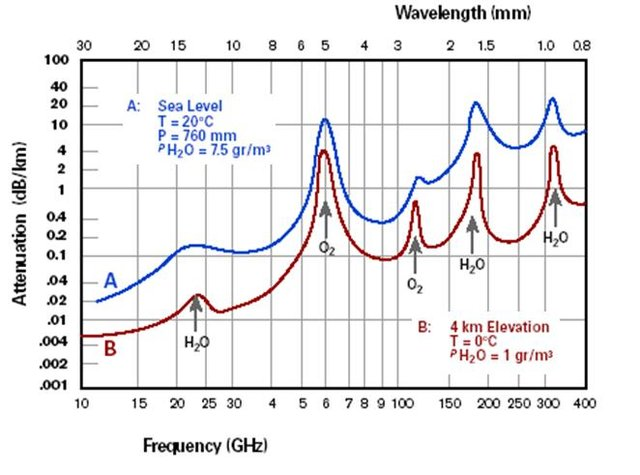
\includegraphics[width=0.8\textwidth]{res/atm-absorp.jpg}
    \caption{Atmospheric absorption in dB per kilometer, from \cite{e-band-ammar}}
    \label{fig:atmospheric-abs}
\end{figure}



\begin{table}[]
    \begin{tabular}{cllll}
    \hline
    {\ul \textbf{Case}} & \multicolumn{1}{c}{{\ul \textbf{Orbit}}} & \multicolumn{1}{c}{{\ul \textbf{Terminal}}} & \multicolumn{1}{c}{{\ul \textbf{Band}}} & \multicolumn{1}{c}{{\ul \textbf{Polarization Reuse}}} \\ \hline
    1  & GEO      & VSAT     & Ka & Disabled \\ \hline
    2  & GEO      & VSAT     & Ka & Enabled  \\ \hline
    3  & GEO      & VSAT     & Ka & Enabled  \\ \hline
    4  & GEO      & Handheld & S  & Disabled \\ \hline
    5  & GEO      & Handheld & S  & Enabled  \\ \hline
    6  & LEO-600  & VSAT     & Ka & Disabled \\ \hline
    7  & LEO-600  & VSAT     & Ka & Enabled  \\ \hline
    8  & LEO-600  & VSAT     & Ka & Enabled  \\ \hline
    9  & LEO-600  & Handheld & S  & Disabled \\ \hline
    10 & LEO-600  & Handheld & S  & Enabled  \\ \hline
    11 & LEO-1200 & VSAT     & Ka & Disabled \\ \hline
    12 & LEO-1200 & VSAT     & Ka & Enabled  \\ \hline
    13 & LEO-1200 & VSAT     & Ka & Enabled  \\ \hline
    14 & LEO-1200 & Handheld & S  & Disabled \\ \hline
    15 & LEO-1200 & Handheld & S  & Enabled  \\ \hline
    \end{tabular}
    \caption{3GPP scenarios for NTN \label{tab:scenarios}}
    \end{table}

\subsection{NS-3 channel model implementation}

\paragraph{}
Work on a ns-3 module to allow simulations in non-terrestrial scenarios to be properly conducted is already in progress, and considerable effort has been put in the realization of a non-terrestrial channel model\footnote{The code is available at the following repository: \href{https://gitlab.com/mattiasandri/ns-3-ntn/-/tree/ntn-dev?ref_type=heads}{gitlab.com/mattiasandri}}.

The implementation of such channel model required the modification and the creation of some ns-3 classes. This work is extensively described in \cite{Sandri_2023}, while a brief overview is hereby reported.

\subsubsection{Modified classes}
\begin{itemize}
    \item \texttt{ThreeGppChannelModel}: different parameters were introduced in order for this class to be able to correctly characterize the non-terrestrial use case. The large number of \ac{NTN}-related parameters made necessary the use of data structures such as maps to store them, and the mobility model of both the satellite and the \ac{UE} have been integrated in the computation of the small scale parameters returned by the class.
    \item \texttt{GeographicPositions}: class tasked with the various conversions between different coordinates systems such as longitude, latitude and altitude, the Geocentric Cartesian system (also called Earth Centric Earth Fixed or ECEF), and the local tangent plane coordinate system expressing the position in North, East and Up coordinates \cite{wiki_coords}. All those three systems are depicted in Fig. \ref{fig:coord-syst}.
\end{itemize}
\subsubsection{New classes}
\begin{itemize}
    \item \texttt{ThreeGppNTNScenarioChannelConditionModel}: the main task of this class is to store the channel state and condition. Four new classes were written to store the four possible scenarios described by \ac{3GPP}:
    \begin{itemize}
        \item Dense urban,
        \item urban,
        \item suburban,
        \item rural
    \end{itemize}
    \item \texttt{ThreeGppNTNScenarioPropagationLossModel}: once again, four different scenarios are implemented in as many classes. Such classes are tasked with the computation of the total path loss, which includes contributions from the standard free space path loss, atmospheric absorption, scintillation, fading and clutter loss.
    \item \texttt{GeocentricConstantPositionMobilityModel}: mainly helps position \ac{UE}s on the Earth surface in an easier way by allowing it to be input in a more natural coordinate set. Conversions amongst different systems are done using the \texttt{GeographicPositions} class described above.
    \item \texttt{CircularApertureAntennaModel}: a more precise implementation of the default ns-3's parabolic antenna model, this time making use of a newer and more efficient C++ function for the computation of Bessel functions required when considering the radiation pattern of aperture antennas \cite{rad-patterns}.
\end{itemize}




\begin{figure}[ht]
    \centering
    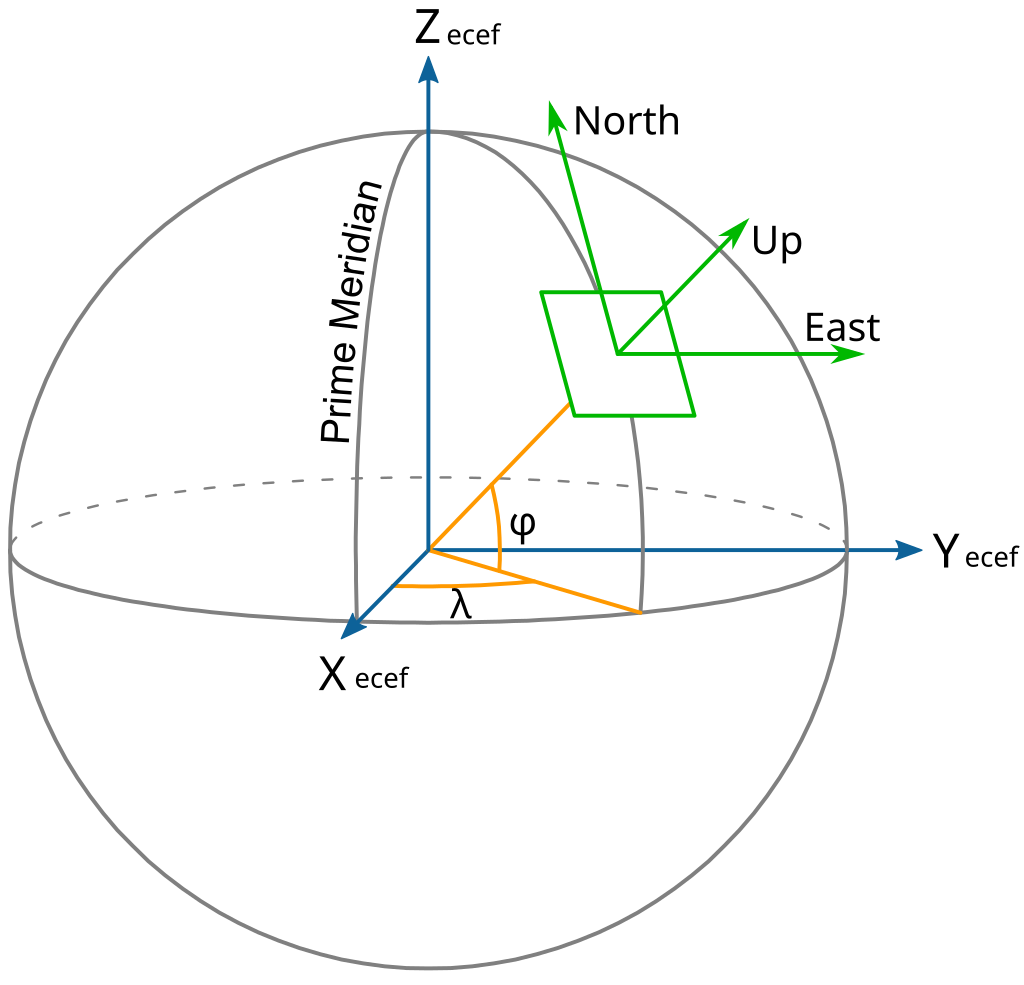
\includegraphics[width=0.5\textwidth]{res/coord_systems.png}
    \caption{Showcase of different coordinates systems \cite{wiki_coords}}
    \label{fig:coord-syst}
\end{figure}

\subsubsection{Use in this work}
\paragraph{}
All the aforementioned implementation is based on the \ac{3GPP} specifications as detailed in the standard \cite{3gpp-tr-38.811}, and the resulting channel model enables full-stack end-to-end simulations considering different \ac{NTN} scenarios \cite{Sandri_2023}.

This work can therefore benefit from an already existing standard implementation of the channel model, a crucial point for its aim of providing a simulation of how the complete \ac{NR} protocol stack would behave in such a challenging scenario. 

\section{Implemented scenario}

This section aims at describing the reference scenario that was implemented in the ns-3 simulator in order to test the \ac{NR} protocol suite in a non-terrestrial communication setting.

\subsection{Network topology}
To conduct the various simulation campaigns, ensuring the reproducibility and the comparability of the obtained results, a reference network topology has been made, and the parameters specified by \ac{3GPP} have been used.

\begin{figure}[ht]
    \centering
    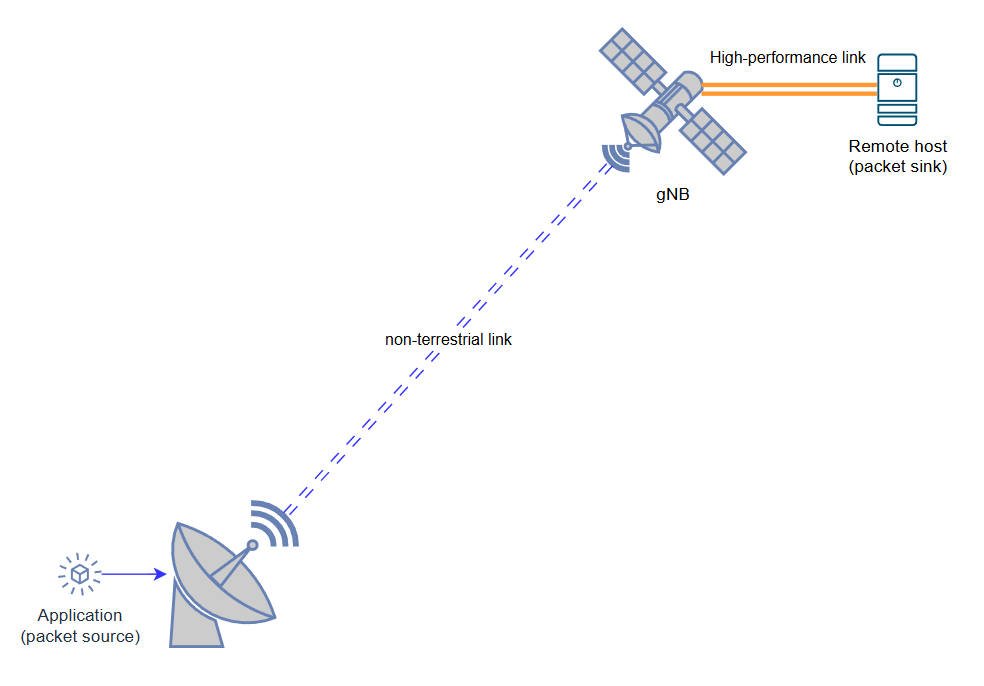
\includegraphics[width=0.8\textwidth]{res/sim-scenario.png}
    \caption{Network simulation scenario}
    \label{fig:sim-scenario}
\end{figure}

The simple network setup is depicted in Fig. \ref{fig:sim-scenario} and it consists of the following elements:
\begin{itemize}
    \item \textbf{Packet source}: application installed on the user equipment that generates packets with a specified periodicity. Both the generation rate and the packets' size can be varied by acting on their respective parameters. All the other variables that can be controlled are listed in the code snippet \ref{code:ue_parameters}
    \item \textbf{UE antenna}: the transmission of data is performed by mean of a \ac{vSAT} antenna placed at the \ac{UE} side. The main parameters of such antenna are found in the code snippet \ref{code:tx_parameters}.
    \item \textbf{Non-terrestrial link}: link connecting the \ac{UE} placed on the ground with the \ac{gNB}. This wireless link is characterized its propagation delay, bandwidth and frequency. However, since the aim of this work is to study the effects of propagation delay on the protocol suite, the bandwidth and frequency remained constant across all the simulations to better isolate the variables that could potentially cause problems. The list of parameters can be found in the code snippet \ref{code:link_parameters}.
    \item \textbf{g-NodeB}: the adopted approach is to incorporate the g-NodeB into the satellite payload, therefore adopting the configuration described in section \ref{sec:onboard-gnb}. This decision was made since the high one-way propagation delay is enough to cause some of the involved protocols to start malfunctioning. Adopting the bent-pipe configuration described in \ref{sec:bent-pipe-payload} would have resulted in effectively doubling the delay between \ac{UE} and \ac{gNB}. The satellite aperture antenna parameters follow the ones specified in the scenario named "10 DL" described in \cite{3gpp-tr-38.821}, and are listed in the code snippet \ref{code:sat_parameters}.
    \item \textbf{High performance link}: link connecting the g-NodeB to the packet sink. This is part of 5G core network, and it shall not be causing any additional problems, since that would be out of the scope of this work. This link was therefore meant to be as close as possible to an ideal one, with a capacity of 100Gb/s, a \ac{MTU} of 1500B and a delay of a single microsecond.
    \item \textbf{Remote host}: packet sink representing the destination node of all the packets generated at the \ac{UE}.
\end{itemize}



\begin{lstlisting}[language=C++, caption=Application and UE configuration parameters, label=code:ue_parameters]
    bool enableNagle = false;  // whether to enable Nagle's algorithm
    bool enableHarq = false;   // whether to enable HARQ protocol
    uint32_t numHarq = 100;    // max number of concurrent HARQ processes
    uint32_t harqTimeout = 10; // timeout for HARQ processes
    bool rrcIdeal = false;     // use ideal version of RRC protocol
    double tcpMinRto = 200;             // minimum TCP RTO
    uint32_t tcpBufSize = 131072 * 100; // TCP buffer size
    double ipv4FrExpTimeout = 200;      // IPv4 fragment expiration timeout
    double perr = 0.1;                  // target error probability when transmitting PHY-level packets

    // Application parameters
    std::string transportPrtcl = "UDP"; // Whether to use UDP or TCP
    uint32_t numPackets = 2000;         // max number of packets to be sent
    double appStartTimeSec = 0.5;       // application start time
    double appStopTimeSec = 5.5;        // application stop time
    double simStopTimeSec = 6;          // simulation stop time
    uint32_t packetSizeBytes = 200;     // application packets' size
\end{lstlisting}

\begin{lstlisting}[language=C++, caption=UE antenna parameters, label=code:tx_parameters]
    // UE Parameters
    double vsatAntennaGain = 39.7;       // dB
    double vsatAntennaDiameter = 0.6;    // meters
    double vsatAntennaNoiseFigure = 1.2; // dB 
\end{lstlisting}

\begin{lstlisting}[language=C++, caption=Satellite antenna parameters, label=code:sat_parameters]
    // Satellite parameters
    double satEIRPDensity = 40;    // dBW/MHz
    double satAntennaGain = 58.5;  // dB
    double satAntennaDiameter = 5; // meters
    double distance = -1;          // height of the satellite in km
\end{lstlisting}

\begin{lstlisting}[language=C++, caption=Non-terrestrial link parameters, label=code:link_parameters]
    uint64_t propDelay = 6;     // propagation delay in ms
    double frequency = 20e9;    // link carrier frequency
    double bandwidth = 400e6;   // link bandwidth
\end{lstlisting}


    %!TEX root = ../main.tex

\chapter{E2E simulation of NR in NTN scenario}
\label{chp:scheduling_problems}

Given the absence of a tool to properly simulate the behavior of the \ac{NR} stack in a non-terrestrial scenario, the first objective of this thesis is to design and implement some modifications to the protocol stack in order to make it work with long propagation delays. The current codebase of ns3-mmWave and ns3-ntn modules only provide separate implementations of the \ac{NR} stack and the non-terrestrial channel model.

The objective of obtaining a base support that permitted \ac{NTN} \ac{NR} simulation was achieved by devising a \ac{NTN} test scenario where we implemented the \ac{NR} stack, launching simulations and examining the results. Each unexpected behavior was documented, analyzed and solved proposing original solutions. Such work was necessary since the current state of the art regarding network simulators is still lacking proper support for the scenario we meant to investigate.

After describing the network topology and scenario that we implemented in the simulator, this chapter focuses on the problems that hampered the ability to correctly send and receive packets. Since many of them involved the scheduler, a brief introduction about the scheduler and its working principles is presented, then each implemented solution is detailed.

\section{Implemented scenario}

This section aims at describing the reference scenario that was implemented in the ns-3 simulator in order to test the \ac{NR} protocol suite in a non-terrestrial communication setting.

\subsection{Network topology}
To conduct the various simulation campaigns, ensuring the reproducibility and the comparability of the obtained results, a reference network topology has been made, and the parameters specified by \ac{3GPP} have been used.

\begin{figure}[ht]
    \centering
    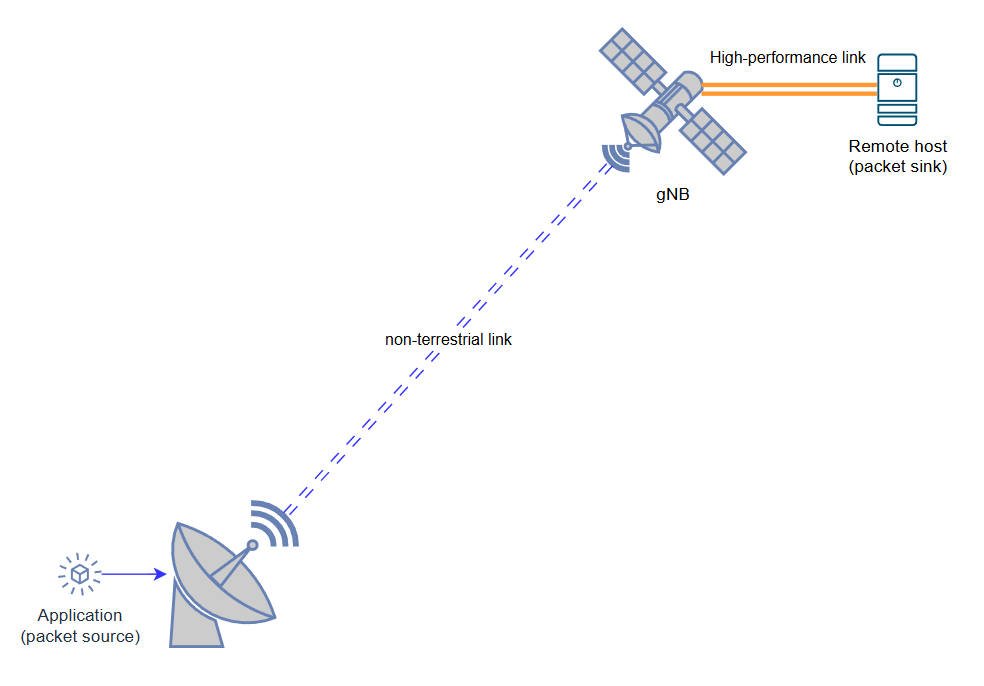
\includegraphics[width=0.8\textwidth]{res/sim-scenario.png}
    \caption{Network simulation scenario}
    \label{fig:sim-scenario}
\end{figure}

The simple network setup is depicted in Fig. \ref{fig:sim-scenario} and it consists of the following elements:
\begin{itemize}
    \item \textbf{Packet source}: application installed on the user equipment that generates packets with a specified periodicity. Both the generation rate and the packets' size can be varied by acting on their respective parameters. All the other variables that can be controlled are listed in the table \ref{tab:params}.
    \item \textbf{UE antenna}: the transmission of data is performed by mean of a \ac{vSAT} antenna placed at the \ac{UE} side. The main parameters of such antenna are found in the table \ref{tab:ue_params}.
    \item \textbf{Non-terrestrial link}: link connecting the \ac{UE} placed on the ground with the \ac{gNB}. This wireless link is characterized its propagation delay, bandwidth and frequency. However, since the aim of this work is to study the effects of propagation delay on the protocol suite, the bandwidth and frequency remained constant across all the simulations to better isolate the variables that could potentially cause problems. The list of parameters can be found in Table \ref{tab:link_params}.
    \item \textbf{g-NodeB}: the adopted approach is to incorporate the g-NodeB into the satellite payload, therefore adopting the configuration described in section \ref{sec:onboard-gnb}. This decision was made since the high one-way propagation delay is enough to cause some of the involved protocols to start malfunctioning. Adopting the bent-pipe configuration described in \ref{sec:bent-pipe-payload} would have resulted in effectively doubling the delay between \ac{UE} and \ac{gNB}. The satellite aperture antenna parameters follow the ones specified in the scenario named "10 DL" described in \cite{3gpp-tr-38.821}, and are listed in the table \ref{tab:sat_params}.
    \item \textbf{High performance link}: link connecting the g-NodeB to the packet sink. This is part of 5G core network, and it shall not be causing any additional problems, since that would be out of the scope of this work. This link was therefore meant to be as close as possible to an ideal one, with a capacity of 100Gb/s, a \ac{MTU} of 1500B and a delay of a single microsecond.
    \item \textbf{Remote host}: packet sink representing the destination node of all the packets generated at the \ac{UE}.
\end{itemize}

\begin{table}[ht]
    \begin{small}
    \begin{tabular}{l|ll}
    \textbf{Parameter name} & \textbf{Description}                       & \textbf{Default} \\ \hline
    enableNagle             & whether to enable Nagle's algorithm        & false            \\
    enableHarq              & whether to enable HARQ protocol            & false            \\
    numHarq                 & number of concurrent HARQ processes per UE & 16               \\
    harqTimeout             & timeout for HARQ processes                 & 100 ms           \\
    rrcIdeal                & use ideal RRC                              & false            \\
    tcpMinRto               & minimum TCP RTO                            & 200 ms           \\
    tcpBufSize              & TCP buffer size                            & 13107200 B       \\
    ipv4FrExpTimeout        & IPv4 fragment expiration timeout           & 200 ms           \\
    perr                    & target error probability for PHY packets   & 0.1              \\
    transportPrtcl          & whether to use UDP or TCP                  & UDP              \\
    numPackets              & max number of packets to be sent           & 2000             \\
    appStartTimeSec         & application start time                     & 0.5 s            \\
    appStopTimeSec          & application stop time                      & 5.5 s            \\
    simStopTimeSec          & simulation stop time                       & 6 s              \\
    packetSizeBytes         & application packets size                   & 200 B           
    \end{tabular}
    \end{small}
    \caption{Application and UE configuration parameters}
    \label{tab:params}
\end{table}



\begin{table}[ht]
    \begin{small}
    \begin{tabular}{l|ll}
    \textbf{Parameter name} & \textbf{Description}             & \textbf{Default} \\ \hline
    vsatAntennaGain         & gain of the vSat antenna         & 39.7 dB          \\
    vsatAntennaDiameter     & diameter of the vSat antenna     & 0.6 dB           \\
    vsatAntennaNoiseFigure  & noise figure of the vSat antenna & 1.2 dB          
    \end{tabular}
    \end{small}
    \caption{UE antenna parameters}
    \label{tab:ue_params}
\end{table}

\begin{table}[ht]
    \begin{small}
    \begin{tabular}{l|ll}
    \textbf{Parameter name} & \textbf{Description}                  & \textbf{Default} \\ \hline
    satEIRPDensity          & EIRP density of the satellite antenna & 40 dBW/MHz       \\
    satAntennaGain          & gain of the satellite antenna         & 58.5 dB          \\
    satAntennaDiameter      & diameter of the satellite antenna     & 5 m              \\
    distance                & orbiting altitude of the satellite    & -1 km           
    \end{tabular}
    \end{small}
    \caption{Satellite antenna parameters}
    \label{tab:sat_params}
\end{table}

\begin{table}[ht]
    \begin{small}
    \begin{tabular}{l|ll}
    \textbf{Parameter name} & \textbf{Description} & \textbf{Default} \\ \hline
    propDelay               & propagation delay    & 6 ms             \\
    frequency               & carrier frequency    & 20E9 Hz          \\
    bandwidth               & link bandwidth       & 400E6 Hz        
    \end{tabular}
    \end{small}
    \caption{Non-terrestrial link parameters}
    \label{tab:link_params}
\end{table}


\section{5G scheduler}
As the name suggests, the main task of the scheduler is to allocate resources to the various connected users in the form of transmission and reception opportunities. In the \ac{NR} standard, the scheduling is dictated by the network and the \ac{UE} has to follow the provided indications \cite{5g-sched-sharetechnote}.

In the \ac{NR} standard, the scheduling process is similar to LTE, with the addition of some new factors and flexibility options. 

\subsection{Frame structure}
The scheduler divides time using four different entities: frames, subframes, slots and symbols. 5G \ac{NR} frame structure is defined in \ac{3GPP} TS 38.211 \cite{3gpp-ts-38.211}. 

Frames always have a duration of 10 ms, while subframes are 1 ms long. Slots and symbols have variable lengths instead, based on the value of a parameter called numerology and represented with the letter $\mu$. Regardless of its time duration, each slot always contain 14 \ac{OFDM} symbols. \cite{gaussianwaves-frame}. 

The $\mu$ parameter can assume integer values in the range $\left[0, 4\right]$, and its value affects the subcarrier spacing and bandwidth, as well as the slot and the symbol durations. Table \ref{tab:mus} contains the values for each supported value of $\mu$ \cite{gaussianwaves-frame}.

\begin{table}[ht]
    \begin{tabular}{l|lllll}
    \textbf{$\mu$} & \textbf{\begin{tabular}[c]{@{}l@{}}Subcarrier spacing\\ $\Delta f = 2^\mu \times 15 \text{kHz}$\end{tabular}} & \textbf{\begin{tabular}[c]{@{}l@{}}Resource block\\ bandwidth\\ $\Delta f \times 12$\end{tabular}} & \textbf{\begin{tabular}[c]{@{}l@{}}Slots per\\ frame\end{tabular}} & \textbf{\begin{tabular}[c]{@{}l@{}}Slot\\ duration\end{tabular}} & \textbf{\begin{tabular}[c]{@{}l@{}}Symbol\\ duration\end{tabular}} \\ \hline
    \textbf{0}  & 15 kHz                                                                        & 180 kHz                                                                               & 10                                                                 & 1 ms                                                             & 71.43 $\mu \text{s}$                                                              \\
    \textbf{1}  & 30 kHz                                                                        & 360 kHz                                                                               & 20                                                                 & 500 $\mu \text{s}$                                                          & 35.71 $\mu \text{s}$                                                              \\
    \textbf{2}  & 60 kHz                                                                        & 720 kHz                                                                               & 40                                                                 & 250 $\mu \text{s}$                                                             & 17.86 $\mu \text{s}$                                                             \\
    \textbf{3}  & 120 kHz                                                                       & 1.44 MHz                                                                              & 80                                                                 & 125 $\mu \text{s}$                                                             & 8.93 $\mu \text{s}$                                                              \\
    \textbf{4}  & 240 kHz                                                                       & 2.88 MHz                                                                              & 160                                                                & 62.5 $\mu \text{s}$                                                            & 4.46 $\mu \text{s}$                                                             
    \end{tabular}
    \caption{Supported numerologies}
    \label{tab:mus}
    \end{table}

Figures \ref{fig:frame1} and \ref{fig:frame2} show the difference in radio frame configuration for $\mu = 0$ and $\mu = 1$. In the first case, each subframe has exactly one slot, while in the second case each subframe contains two slots, the subcarrier bandwidth is doubled and the duration of each symbol halved.

\begin{figure}[ht]
    \centering
    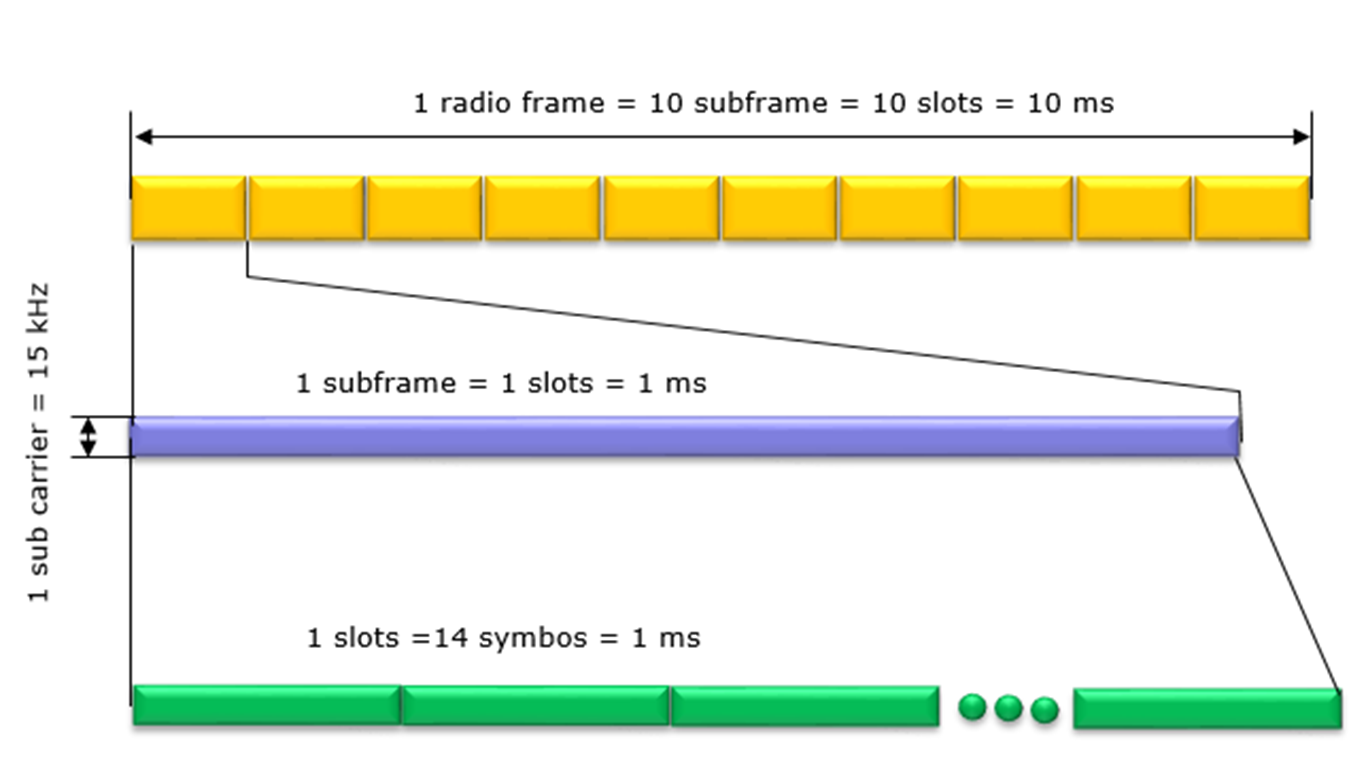
\includegraphics[width=0.8\textwidth]{res/frame-1.png}
    \caption{Radio frame structure for $\mu=0$ \cite{frame-5gnet}}
    \label{fig:frame1}
\end{figure}

\begin{figure}[ht]
    \centering
    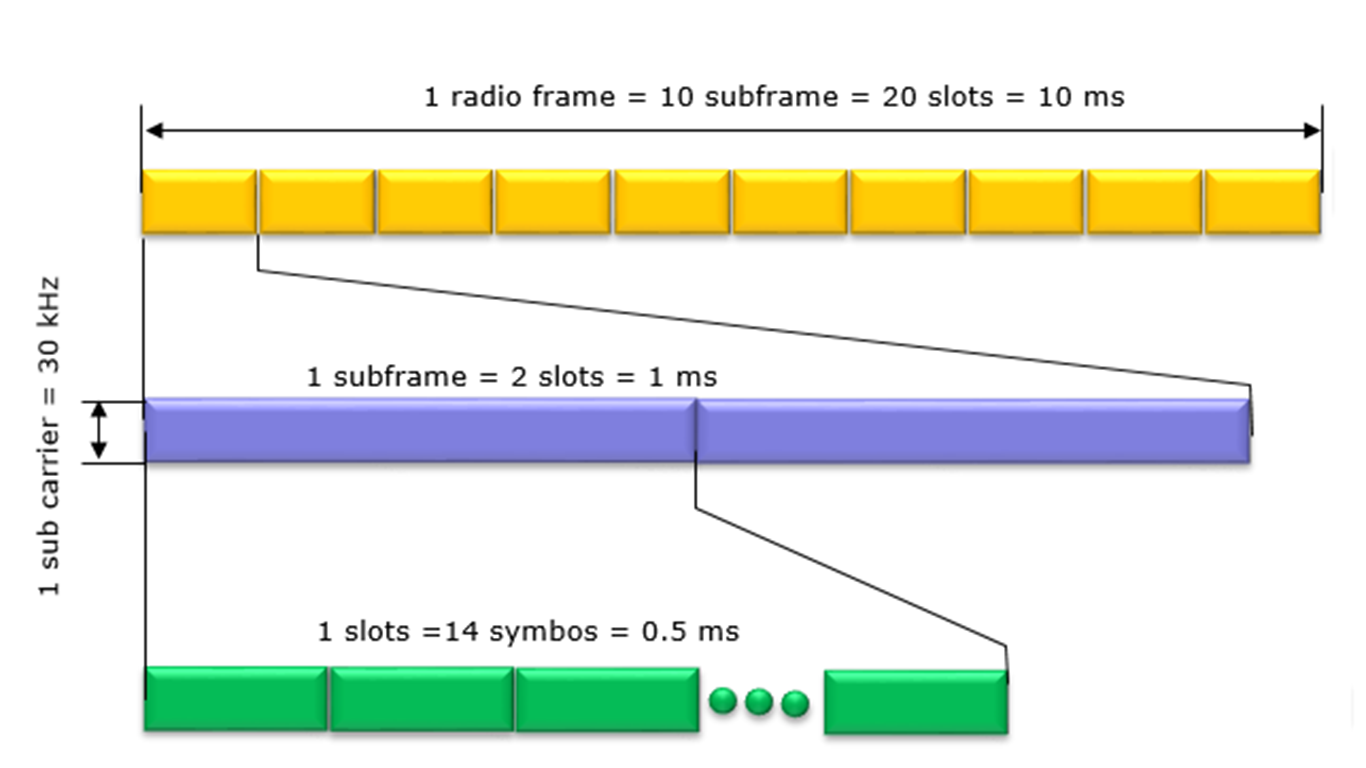
\includegraphics[width=0.8\textwidth]{res/frame-2.png}
    \caption{Radio frame structure for $\mu=1$ \cite{frame-5gnet}}
    \label{fig:frame2}
\end{figure}

\subsection{Dedicated configuration}
Differently from LTE, where a predefined pattern was in place when allocating downlink and uplink slots in a radio frame, in \ac{NR} this is done much more flexibly using a plethora of parameters such as the periodicity of UL and DL transmissions, the number of consecutive DL and UL slots and symbols at the beginning of each pattern and more \cite{5g-sched-sharetechnote}

In LTE, once a subframe is flagged as either UL or DL, all of its symbols are used for the allocated purpose, while \ac{NR} enables symbol-level scheduling, meaning that we don't need to use every symbol within a slot, and each slot can be further divided in groups of symbols reserved for UL and DL. The term slot format indicates how each symbol within a slot is used \cite{frame-5gnet}. 


\subsection{Propagation delay and differential delay}
\paragraph{}The important key concept is that the scheduler shall account for the propagation delay. While in terrestrial communications a guard period of six symbols when switching from downlink communications to uplink communications is sufficient to account for the delay in a few km-radius cell, and timing advance commands can account for the different propagation delays experienced by users located in the center of the cell and users located in the cell edge \cite{gsma-5g-tdd-sync}, the same cannot be said for non-terrestrial use cases, where the distances that come into play are much longer, therefore delays are higher.

Consider the case depicted in Figure \ref{fig:diff-delay} from \cite{preamble-detection-chougrani}. For a \ac{LEO} satellite orbiting at 600Km, cell diameter of 82Km and elevation angle of 45°, the maximum differential round-trip delay of UE2 with respect to UE1 is of $370\mu s$ \cite{preamble-detection-chougrani}. On the other hand, a 3km-radius cell experiences a maximum round-trip differential delay of $2*\text{radius}/c \approx 10\mu s$

\begin{figure}[ht]
    \centering
    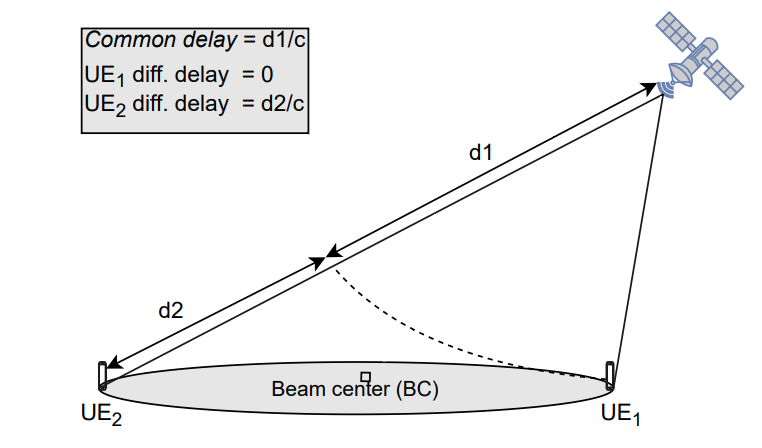
\includegraphics[width=0.8\textwidth]{res/diff-delay.png}
    \caption{Differential delay for \ac{NTN}, courtesy of \cite{preamble-detection-chougrani}.}
    \label{fig:diff-delay}
\end{figure}


\section{Accounting for propagation delay in scheduling}
\label{sec:pd-sched-acc}

\subsection{Problem description}
\label{ss:propdelay-problem-desc}
\paragraph{}
The first encountered problem while implementing a non-terrestrial communication scenario in the simulator was the inability of the scheduler to account for the propagation delay when allocating radio resources to the connected user equipment on the ground.

The implementation of the 5G scheduler in ns-3 is designed to allocate resources less than a single subframe in advance, and since each subframe has a duration time of 1ms, the resource grant was already expired by the time it was able to reach the \ac{UE}, since it was referring to a past subframe.

\paragraph{Example} Consider a scenario with a propagation delay $\tau_p$ of 6ms, corresponding to a satellite at an altitude of 1800 km. The \ac{UE} sends a request for uplink resources at time $t_0$ since it has some data to send. In the standard scheduler implementation, assuming an ideal transmission, the \ac{gNB} would receive such request at $t_0+\tau_p=6\textit{ms}$. Provided that other transmissions have not been scheduled yet, the \ac{gNB} grants the \ac{UE} the possibility to transmit in the following subframe, which will start after 1ms at $t_0+\tau_p+t_{\textit{SF}}=7\textit{ms}$. The grant that allows the \ac{UE} to transmit at $t=7\textit{ms}$ is ideally transmitted by the \ac{gNB} as soon as it receives the request, therefore at $t=6\textit{ms}$. However, this grant will reach the \ac{UE} only after another propagation delay, at $t_0+2\tau_p=12\textit{ms}$, when the transmission opportunity would already have expired.

\subsection{Implemented solution}
\label{ss:propdelay-problem-sol}
The implemented solution assumes that the scheduler has knowledge of an estimation of the propagation delay, that can be obtained through the use of probe signals and basing on previously measured values. This is a reasonable assumption since systems such as GPS already rely on a precise estimation of the delay between the user on the ground and the satellite.

The scheduling then proceeds as normal with the only difference being that the information regarding the propagation delay is used to postpone the allocated symbols. 

\paragraph{Example} Consider a scenario with propagation delay $\tau_p$ of 5 slots (roughly 1,2ms). The new implementation of the scheduler accounts for the propagation delay by allocating the first available slot after $\tau_p$, so the time for the grant to reach the \ac{UE} is accounted for, and the \ac{gNB} marks the slot after $2\tau_p$ as reserved.

The last part of reserving a different slot is not as immediate. However, this mechanism needs to be in place because of the behavior depicted in Figure \ref{fig:scheduler-allocations-pd} and hereby detailed. In this scenario, the numerology $\mu$ is 2, therefore each subframe contains 4 slots.


\begin{itemize}
    \item \ac{UE} sends the scheduling request to \ac{gNB} at frame 1, subframe 0, slot 0.
    \item The \ac{SR} reaches the \ac{gNB} after $1\tau_p$ of 5 slots and the \ac{UE} is scheduled to transmit at frame 1, subframe 2, slot 2 since there is some noticeable propagation delay.
    \item The \ac{SR} reaches the \ac{UE} at frame 1, subframe 2, slot 2, and the \ac{UE} can transmit right away.
    \item The packet reaches the \ac{gNB} after another $\tau_p$, hence the base station needs to know that it cannot schedule other transmissions to take place in this slot, otherwise interference and collisions may arise.
\end{itemize}

\begin{figure}[ht]
    \centering
    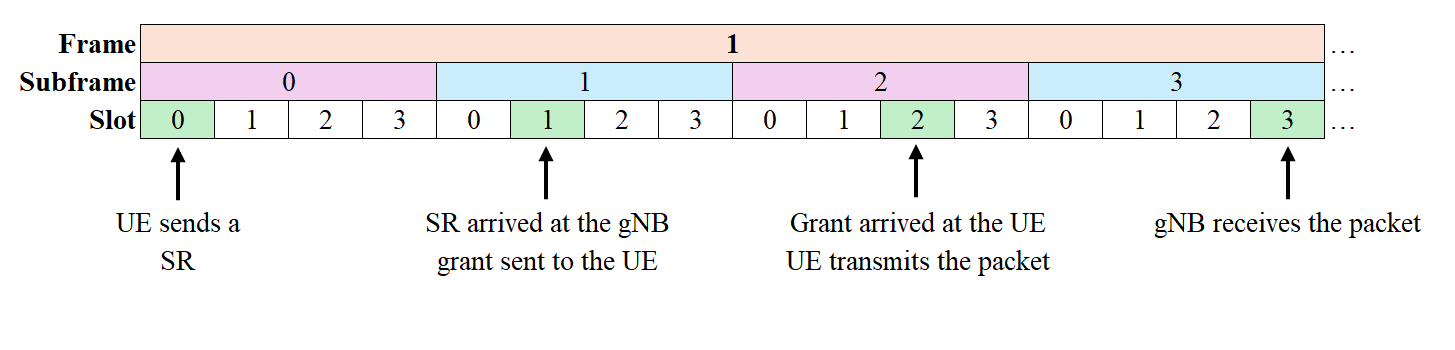
\includegraphics[width=0.9\textwidth]{res/scheduler-allocation-pd.png}
    \caption{Difference between allocated slot and gNB reception}
    \label{fig:scheduler-allocations-pd}
\end{figure}

\paragraph{ns-3 implementation}
This solution has been implemented as a modification to the classes \texttt{MmWaveFlexTtiMacScheduler} and \texttt{MmWaveEnbPhy}, that now account for delayed responses of previously scheduled transmissions when allocating new slots.

The classes \texttt{MmWaveUePhy} and \texttt{MmWavePhy} have also been modified to allow access to the propagation delay parameter of the physical channel.

\section{BSR timer}
\label{sec:bsr-timer}
After implementing the solution discussed in the previous point in the ns-3 network simulator, allowing the communication to take place, some other irregularities were found regarding the periodic \ac{BSR} timer, as described in the following. 

\subsection{Problem description}

\paragraph{Reduced latency}

Figure \ref{fig:lat-saw} shows a rather peculiar trend regarding latency. The expected result was a linear increase in latency with a slope of 3, where every packet arrived at the destination after three times the propagation delays. The reasoning behind this expectation was that every packet generated by the application should have triggered a scheduling request received by the \ac{gNB} after $\tau_p$, a grant to be emitted requiring another $\tau_p$ to reach the \ac{UE}, and finally the transmission to be received by the \ac{gNB} after the third propagation delay (with the assumption of ideal transmission).

The observed pattern did not match any of the expectations. The output obtained from the simulation campaign showed a nonlinear saw tooth behavior presenting values that consistently stayed under the expected $3\tau_p$ threshold value, shown in green in Fig. \ref{fig:lat-saw}.

\begin{figure}[ht]
    \centering
    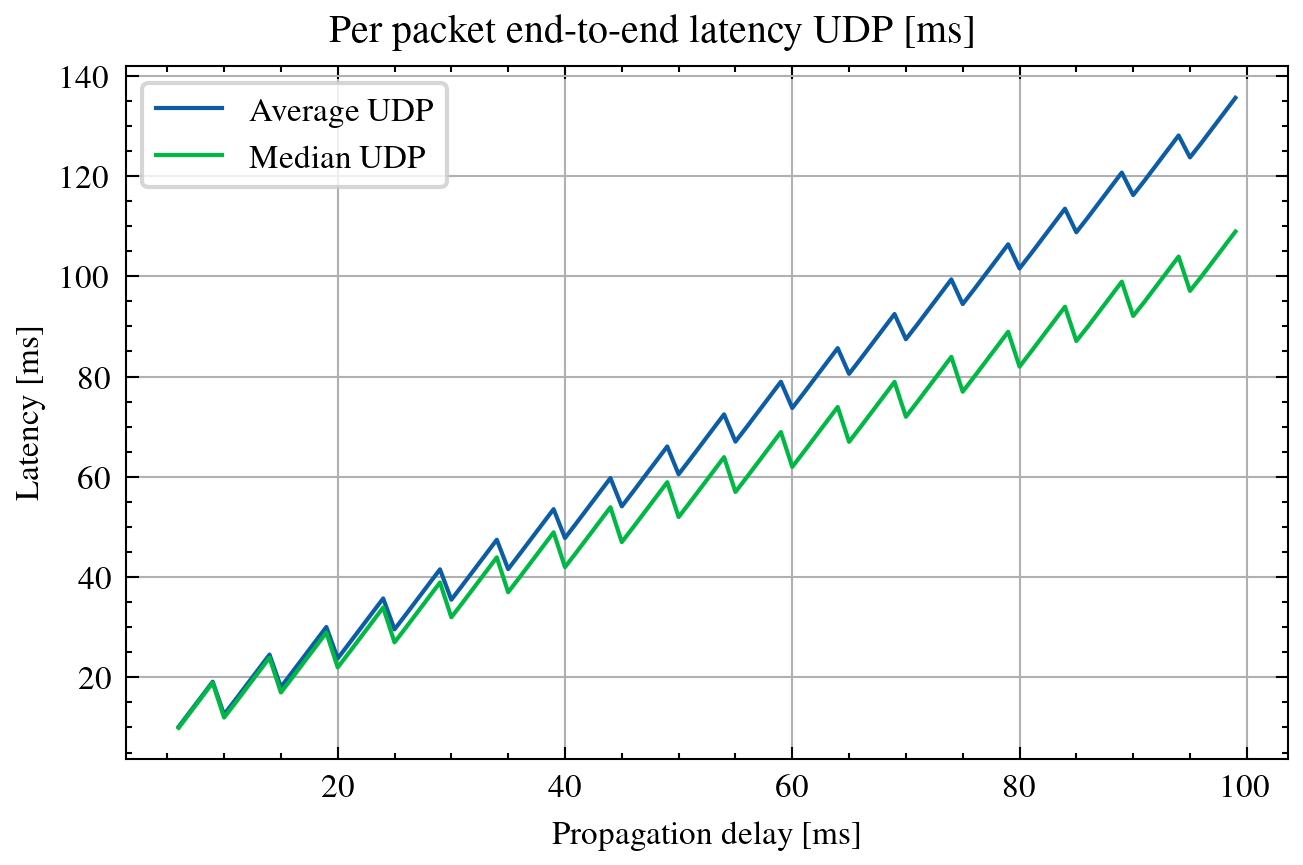
\includegraphics[width=0.8\textwidth]{res/lat-udp-saw.png}
    \caption{E2E latency vs. propagation delay with periodic \ac{BSR}}
    \label{fig:lat-saw}
\end{figure}

\paragraph{Periodic buffer status reports} Further investigation on the subject allowed identifying numerous buffer status reports sent from the \ac{UE} to the \ac{gNB} at regular intervals of 10ms, even when no new packets were produced by the application.

Buffer status reports are messages that the \ac{UE} uses to communicate to the \ac{gNB} the status of its transmission buffer. Every new packet arriving to the transmission buffer of the \ac{UE} changes its status and a new \ac{BSR} is sent, containing information such as the number of queued packets and their size. Upon reception, the \ac{gNB} can grant the \ac{UE} some resources to transmit part or all of the contents of its buffer. Each \ac{BSR} is therefore interpreted as a \ac{SR}.

This behavior happens because the implementation of 5G \ac{MAC} layer includes a periodic \ac{BSR} that the \ac{UE} sends to the \ac{gNB} as long as the transmission buffer contains some pending data.
The details of this mechanism are documented in Section 5.4.5 of the standard \cite{etsi-mac-specification}, where it is also stated that the default interval between those periodic \ac{BSR} is of 10ms.

This characteristic was meant to act as a safeguard against lost scheduling requests, and does not account for the propagation delay at all. The \ac{UE} therefore continues to send additional buffer status reports at regular 10ms intervals even though the previous ones were not lost, but still travelling towards the base station because of a (very long) in-fligh propagation delay.

\paragraph{}
Figure \ref{fig:diagram-wasted-capacity} illustrates this behavior. The arrival at the \ac{UE}'s application buffer of packet p1 at time $t=0$ triggers the transmission of a first \ac{SR}. Since the hereby depicted scenario has a propagation delay of 20ms, the \ac{SR} will arrive at the g-NodeB at time 20ms. However, the \ac{BSR} timer expires at $t=10\text{ms}$ by default, so during a single round-trip time the \ac{BSR} is repeated four times. The green arrows marked with a capital G denote all the grants issued to the \ac{UE}. Only one of the four depicted will actually be used by the \ac{UE} for the intended packet, effectively wasting three out of four transmission opportunities that could have been allocated to other users waiting to transmit.

\begin{figure}[ht]
    \centering
    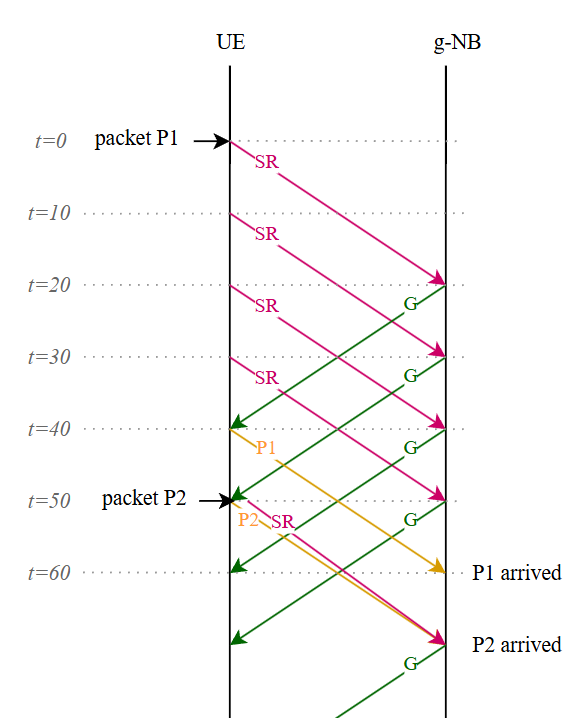
\includegraphics[width=0.5\textwidth]{res/diagram-wasted-grants.png}
    \caption{Packet diagram with periodic \ac{BSR}}
    \label{fig:diagram-wasted-capacity}
\end{figure}

The reduction in latency was observed because newly arrived packets could, in certain situations, make use of the resource grants that were meant for the previous packets but have yet to arrive at the \ac{UE}. Consider the arrival of another packet (P2) at the\ac{UE}'s application buffer. in figure \ref{fig:diagram-wasted-capacity}. It triggers another \ac{SR}, but a grant (originally intended for and trigger by P1) is received immediately after, therefore allowing for an immediate transmission of P2, which will experience a latency of only a single propagation delay. This instantaneous grant is nothing but the result of the previous \ac{SR} storm originated from the \ac{UE} itself.

While this can present some beneficial aspects such as the reduced overall latency, it originates from a behavior that is outside the original design intentions. Moreover, this approach is particularly greedy, leading to wasted capacity.

\subsection{Implemented solution}

After the successful identification and characterization of the problem, the  solution consisted of the implementation of a simple adaptive algorithm that would dynamically set the \ac{BSR} timer to a value of twice the propagation delay plus a constant of 4ms that accounts for the processing times as well as any possible delay. The constant was chosen accounting for the characteristics of the link, the packets transmission times as well as processing times.

\paragraph{ns-3 implementation}
Modifications were made to the \texttt{LteRlcUm} class to expose the buffer status report timer parameter using the ns-3 attribute framework, therefore permitting its dynamic adjustment based on the propagation delay. 

This allowed the simulation manager software to test different values of the \ac{BSR} timer, as well as a more standardized way of setting its value without changes to the source code. Figure \ref{fig:lat-improved} shows the result of our implementation. Latency now closely follows the expected results, only presenting a marginal increase due to the non-null transmission and processing times.

\begin{figure}[ht]
    \centering
    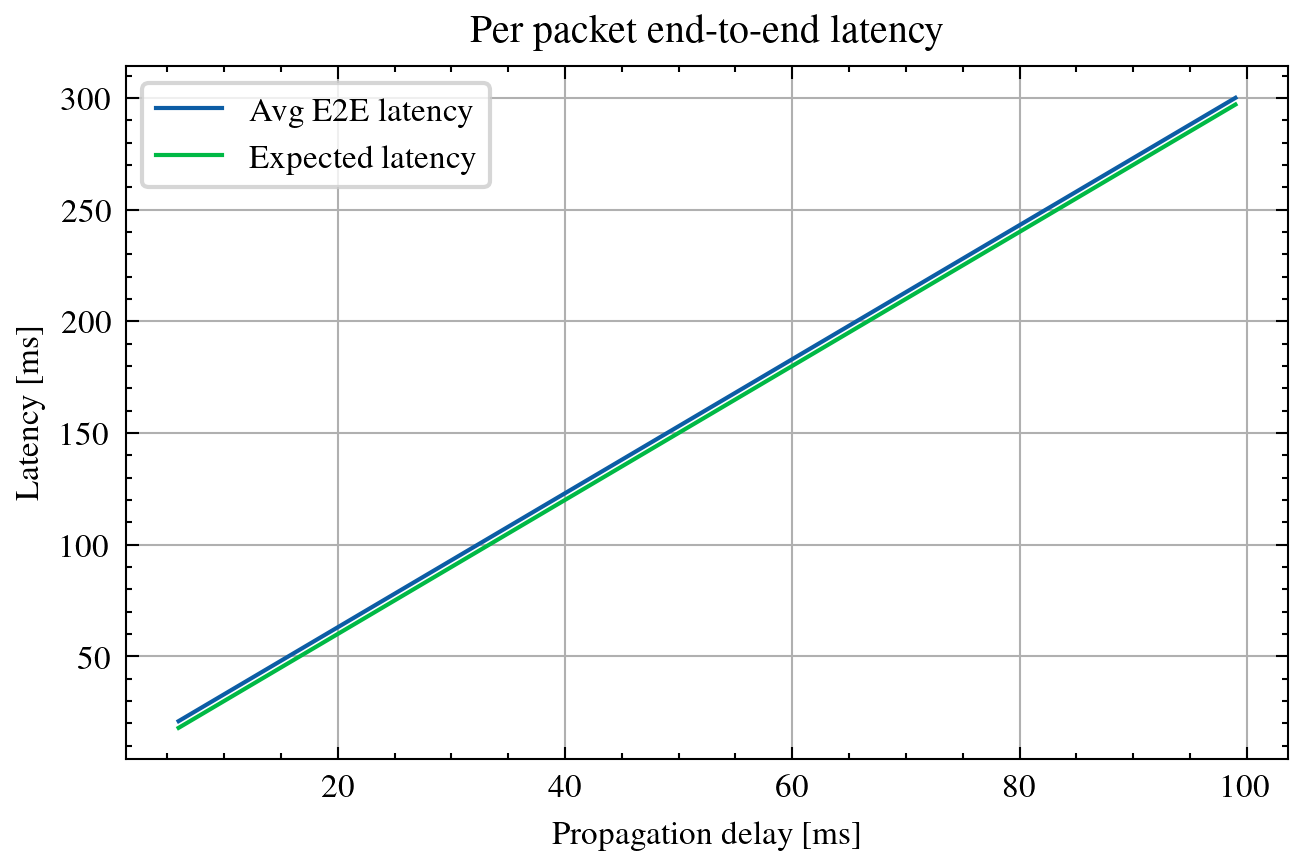
\includegraphics[width=0.8\textwidth]{res/lat_sched_after.png}
    \caption{E2E latency vs. propagation delay with implemented solution}
    \label{fig:lat-improved}
\end{figure}


\paragraph{Area of potential improvement}
The implementation of the aforementioned solution, however, while working as intended, had the expected but unwelcomed effect of increasing the overall latency of the system, since all the additional grants required by previous packets that newly generated ones could exploit were no longer available.

This unexpected problematic behavior of wasted transmission opportunities accidentally also unveiled the potential of preemptively transmitting additional scheduling requests, so that future packets could be sent with a lower latency.

If implemented correctly, the \ac{UE} could adopt a predictive approach towards its traffic needs for the near future basing its estimates on the type of application, and send the \ac{gNB} scheduling requests for packets that have yet to be generated.

\section{Inflated BSR}
\label{sec:inf-bsr}

\subsection{Problem description}
Another problem occurred when the interval between the packets generated by the application, i.e. the packets interarrival time, was smaller than a single round-trip time. 

\paragraph{}
The arrival of each packet automatically triggers the transmission of a scheduling request by the \ac{UE}. However, each request is made for the whole transmission buffer. This causes a problem when many packets arrive before the \ac{gNB} has the chance to respond with the appropriate resource grant.

Referring to Figure \ref{fig:inflated-bsr-diag}, we can see that the arrival of P1 in the transmission buffer of the \ac{UE} triggers the transmission of a \ac{SR} for a single packet. The second packet P2 arriving after 10ms triggers another request, however this second request is cumulatively made for the full buffer length, regardless of the fact that the first \ac{SR} is still pending. This is denoted by the writing "SRx2". Packets P3 and P4 behave in the same way, triggering requests for the allocation of three and four additional packets respectively.

Finally, the grants start arriving at the \ac{UE}. The first 1-packet grant allows for the transmission of P1, while the second grant, requested for two packets, allows for the transmission of packets P2 and P3. The third grant, which corresponds to a previous request for 3 packets and could therefore allow the transmission of 3 packets, can now only be used by P4, wasting 2/3 of its potential capacity. 

The last grant, that would allow the \ac{UE} to transmit 4 consecutive packets, is completely wasted since the send buffer is now empty.

\begin{figure}[ht]
    \centering
    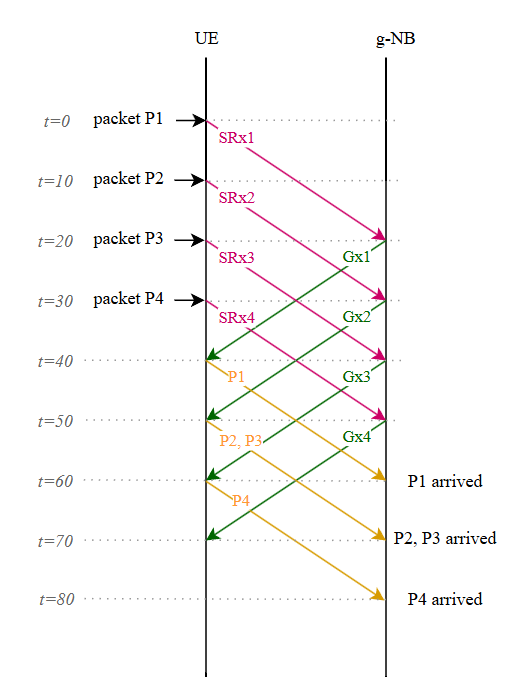
\includegraphics[width=0.5\textwidth]{res/diagram-inflated-bsr.png}
    \caption{Packet diagram for interarrival times smaller than propagation delay}
    \label{fig:inflated-bsr-diag}
\end{figure}
\begin{figure}[ht!]
    \centering
    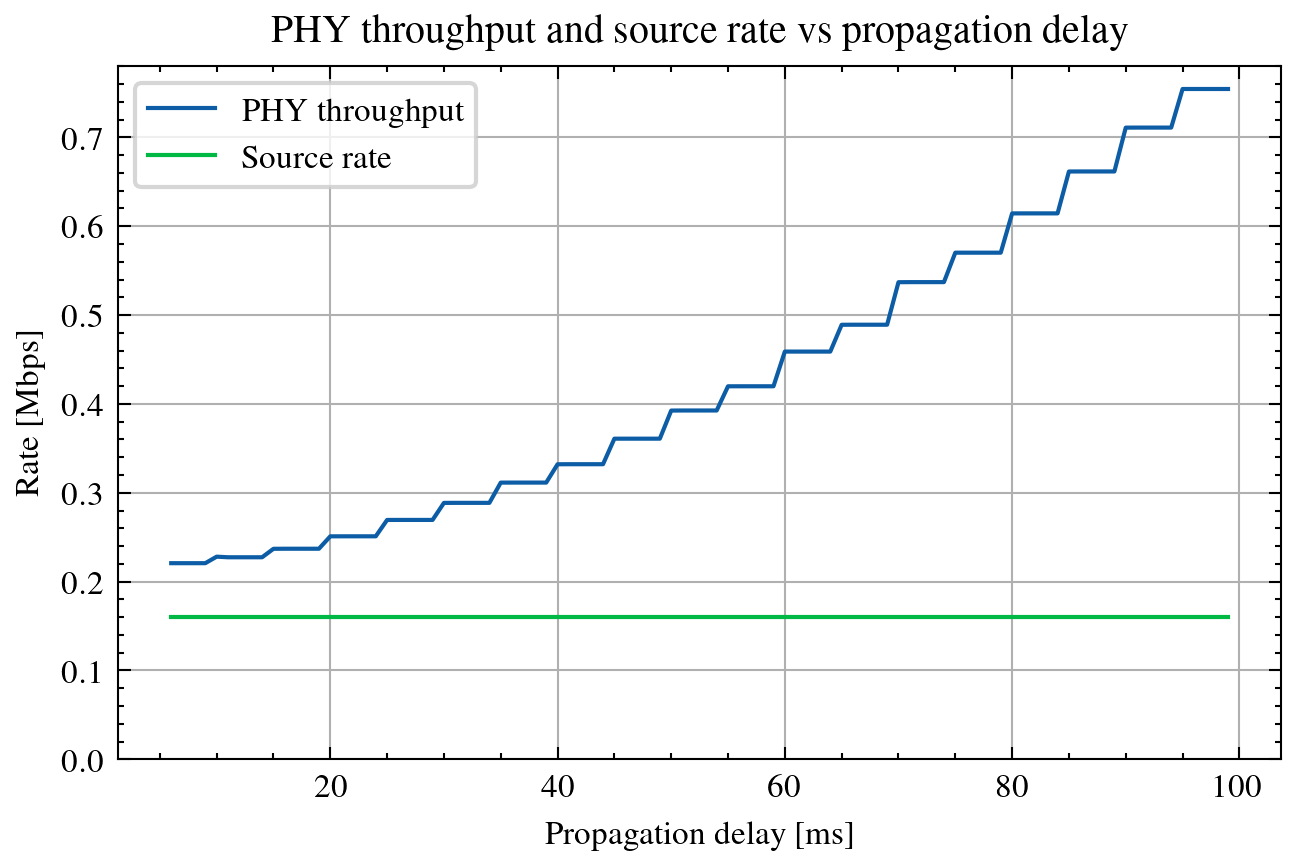
\includegraphics[width=0.8\textwidth]{res/phy-thr-udp-runaway-new.png}
    \caption{Physical throughput and application source rate vs. propagation delay with inflated requests}
    \label{fig:phy-thr-runaway}
\end{figure}
\paragraph{Repercussions}
The described behavior caused the physical throughput to be significantly higher than the application source rate, since the physical throughput metric counts all the capacity assigned to the \ac{UE}, even though part of it might be just padding. Figure \ref{fig:phy-thr-runaway} shows the observed physical throughput for a constant source rate of 160Kb/s. The area between the two lines indicates that a lot of radio resources are being wasted to transmit few data. All the unused space in the grants that the \ac{UE} receives is filled with padding, that counts as physical throughput but is useless at the higher levels. The growing trend when the propagation delay increases happens because the \ac{SR} and grants take more time to arrive at their destinations, and the \ac{UE} keeps sending inflated \ac{BSR}s for more time, further contributing to waste more resources.



\subsection{Implemented solution}

Various different approaches could be undertaken in order to tackle this problem. Nonetheless, a comprehensive study detailing upsides and downsides of each of them is outside the scope of this thesis. 

The implemented solution consists of a modification to the \ac{SR} algorithm that limits the requests to only account for the newly received data, therefore disabling the cumulative behavior. If a packet is already in the buffer when a new one arrives, the scheduling request only asks the size of the second packet to be allocated.
\begin{figure}[ht]
    \centering
    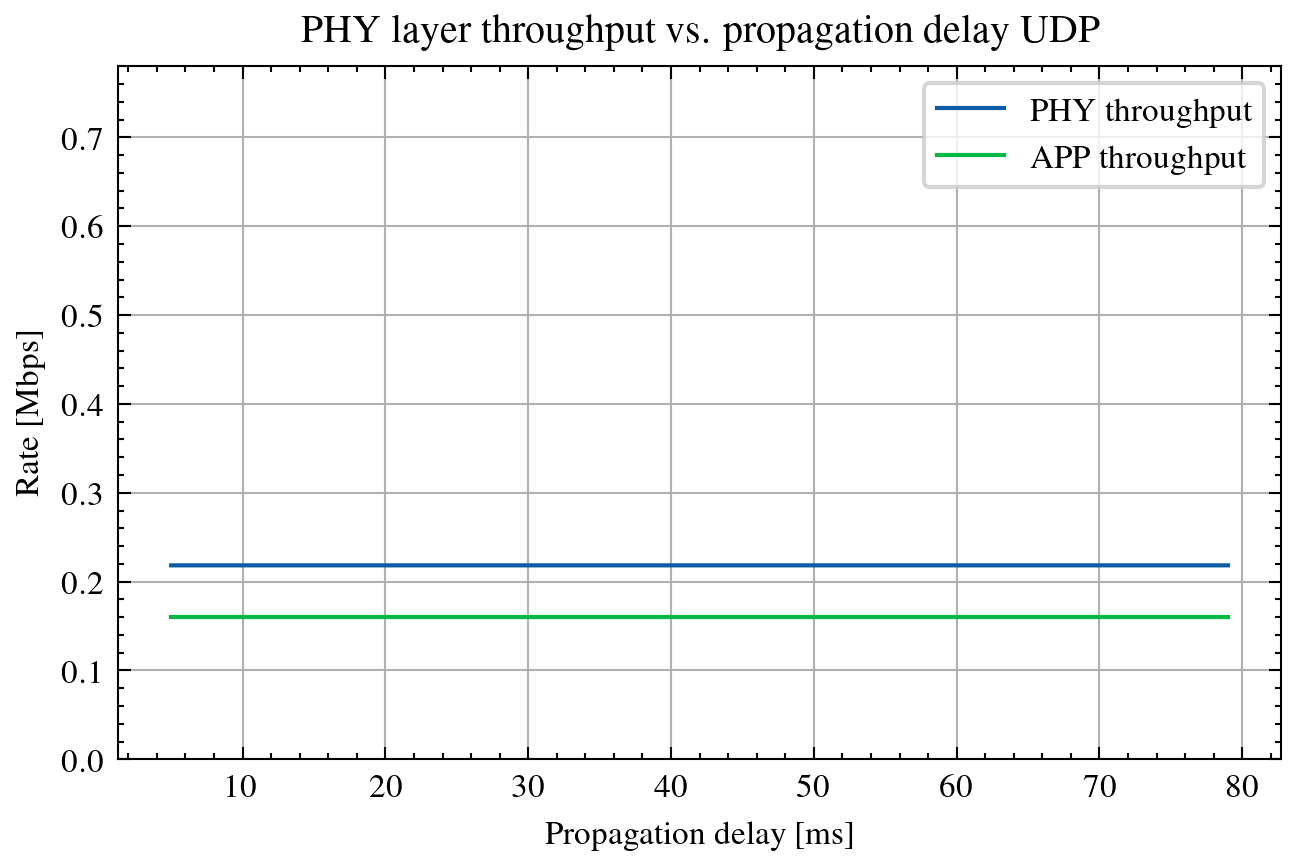
\includegraphics[width=0.8\textwidth]{res/phy_thr_new.png}
    \caption{PHY throughput vs. propagation delay with implemented solution}
    \label{fig:phy-thr-after}
\end{figure}

\begin{figure}[ht!]
    \centering
    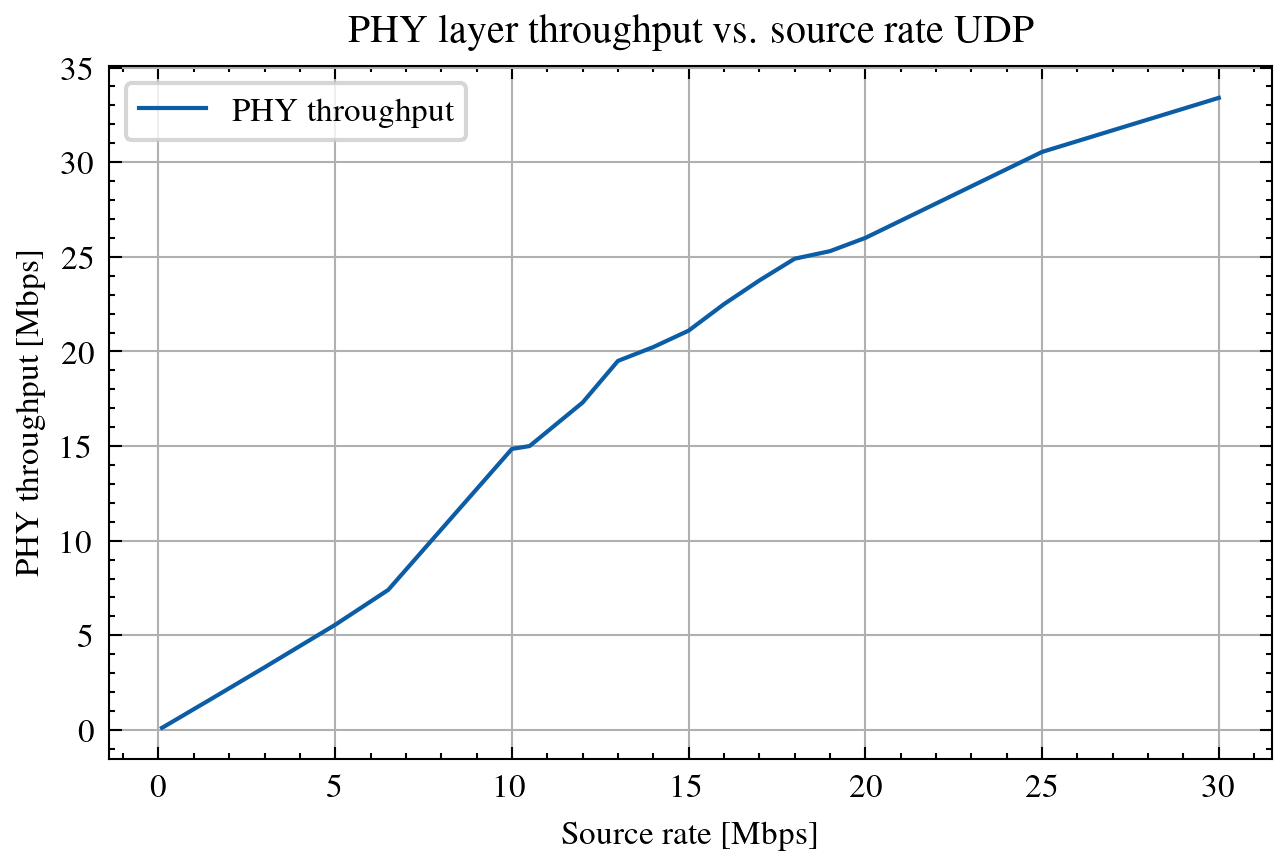
\includegraphics[width=0.8\textwidth]{res/phy_vs_sr.png}
    \caption{Physical throughput vs. source rate}
    \label{fig:phy-vs-sr}
\end{figure}
The effectiveness of the implemented solution can be seen in Figure \ref{fig:phy-thr-after}, showing that the physical layer throughput remains constant as the propagation delay increases, as reasonably expected since the source rate is constant throughout the simulation.



Finally, Figure \ref{fig:phy-vs-sr} shows the behavior of the physical throughput as the application source rate increases. Note that the application rate is always smaller than the physical throughput. This happens because the \ac{TB} that the \ac{gNB} assigns to the \ac{UE} have dimensions that can only be integer multiples of the size of an OFDM symbol, therefore each \ac{TB} can be slightly larger than the actual application-level packet. Furthermore,physical throughput also accounts for protocol overheads, otherwise discarded in the computation of the application source rate.

\paragraph{ns-3 implementation}
The method responsible for the cumulative buffer status reports is \texttt{DoReportBufferStatus()} in the \texttt{LteRlcUm} class, therefore it was modified to only account for the newly arrived data when sending a \ac{SR}.


\section{Reordering timer}
\label{sec:reord-timer}

\subsection{Problem description}
\paragraph{Fragmentation}
The packets interarrival times are not necessarily multiples of the propagation delay, and the resources that the g-NodeB grants to the \ac{UE} are usually a few bytes larger than the packet size. This happens because, even though 5G scheduling can be done on a much finer granularity than 4G scheduling, the base station still cannot grant values that are smaller than a single symbol, so the general rule is to allocate the minimum number of symbols whose cumulative size is greater or equal to the requested allowance.

This misalignment between packet size and transmission opportunities allows for packets to be split in smaller pieces. If two packets of 200B each are waiting in the buffer to be transmitted, and a resource grant for 220B arrives at the \ac{UE}, the first packet can be completely transmitted, but it would be wasteful not to use also the 20 additional bytes that were granted, so the second packet is split and only its first bytes are transmitted. The remaining ones will wait for the next opportunity.

\paragraph{PDCP}
The detailed implementation of the \ac{PDCP} layer can be found in the \ac{3GPP} technical specification \cite{pdcp-spec-3gpp}, while the diagram describing its functionality has been reported in Figure \ref{fig:pdcp-functionalities}. This layer offers reordering services by employing a sequence number, integrity protection and ciphering if the packet in question is associated to a \ac{PDCP} \ac{SDU}, and duplication and routing when operating split bearers.

\begin{figure}[ht]
    \centering
    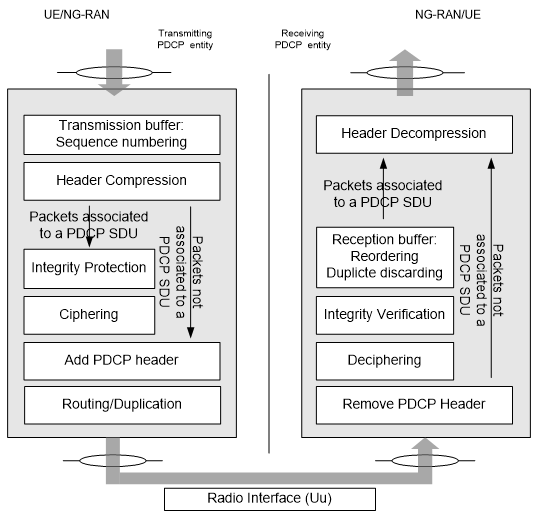
\includegraphics[width=0.7\textwidth]{res/pdcp-functionality.png}
    \caption{PDCP diagram \cite{pdcp-spec-3gpp}}
    \label{fig:pdcp-functionalities}
\end{figure}

The observed problem, as the propagation delay increases, is related to an expiring timer when reassembling the packets at the \ac{PDCP} layer. The so-called reordering timer (t-reordering), which despite the name also affects the recomposition of fragmented packets, is not configured for the use in a non-terrestrial scenario, and it regularly expires due to the long propagation delay before the second half of the packet managed to arrive, leading to the discard of otherwise good packets.

This re-ordering functionality of \ac{PDCP} layer is in place to ensure a sequential delivery of packets to the upper layers. In case of missing packets, the approach is to wait until either the packets arrive or the reordering timer expires \cite{efficient-reassembly-pdcp}. It was observed that this timer also started when the \ac{PDCP} layer was waiting for the arrival of the second part of a fragmented packet. However, due to the high propagation delay, the second half of the packet did not arrive before the timer expiration, leading to the packet being discarded.

Should the reordering timer be set too high, it may cause additional latency, and, if set too low, it might cause many packets to be discarded, as in the case that was hereby simulated.


\subsection{Implemented solution}
Since the use of timers always bears trade-offs depending on their value, in this case either being a higher latency or a higher packet discard ratio, there can not be a one-fits-all approach: the differences in propagation delays between satellites orbiting at different altitudes are so drastic that the implementation of a single default value would lead to suboptimal performances in every possible scenario. 

The class \texttt{LteRlcUm} was therefore modified to expose the \texttt{ReorderingTimer} parameter, allowing to easily set its value using the ns-3 attribute framework, similarly to the approach undertaken while solving the previous problem. This in turn permitted to set the timer to the value of the propagation delay plus a small constant accounting for processing delays for each simulator run.
    %!TEX root = ../main.tex

\chapter{Optimizing NR HARQ for NTNs}
\label{chp:harq}
The previous chapters describe how we developed a working simulator for \ac{NR} stack in a non-terrestrial scenario, the encountered problems and the proposed solutions. This chapter focuses on the improvement of \ac{NR} \ac{NTN} performances, in particular regarding the \ac{HARQ} protocol, that has been identified by \ac{3GPP} as prone to failure due to the high propagation delays of \ac{NTN}s. Our aim is to verify its current status and performances in \ac{NTN}s, and optimize its behavior by designing and implementing some original modifications.

After a brief overview of \ac{HARQ} key concepts, the problems with \ac{HARQ} that emerged during the simulation campaing are presented, critically evaluated and followed by a detailed explanation of the implemented solutions.

\section{HARQ overview}
The main objective of telecommunication networks is the transfer of information between different actors. Modern systems aim at an efficient usage of the available resources, while trying to meet all the necessary requirements of the application that is generating the data to be transferred. 

The \ac{HARQ} protocol hereby described helps achieve a more efficient use of the available resources when errors occur, using an intelligent system of retransmissions that, in turn, reduces the error rate at the expense of a higher latency.

The main building blocks of \ac{HARQ} are \ac{ARQ} and \ac{FEC}. The role of \ac{ARQ} is to automatically request the retransmission of the whole packet when the receiver detects the presence of errors, or when packets are not received at all, while \ac{FEC} is tasked to correct such errors using redundancy bits added to the packet by the transmitter. The joint operation of those two protocols makes the foundation of \ac{HARQ}, currently in use in all the most popular network standards such as 4G, Wi-Fi and 5G \cite{3gpp-38-series}. \ac{HARQ} peculiarity resides in the fact that it avoids the retransmission of the whole packet in case of errors, preferring to send additional redundant information to help the decoding process.

\section{Concurrent processes limit}
\label{sec:harq-conc-proc}

One of the problems of \ac{HARQ} highlighted by the \ac{3GPP} technical report \cite{3gpp-tr-38.811} in the \ac{NTN} scenario regards the maximum number of concurrent \ac{HARQ} processes. 

\subsection{Problem description}
The details of \ac{HARQ} protocol implementation in the 5G \ac{NR} standard is extensively treated in many publications such as \cite{harq-wireless-communications-survey}. However, for the purpose of understanding what is a \ac{HARQ} process and how it affects the throughput in a non-terrestrial scenario, we only give a brief overview in the following paragraphs.

\begin{figure}[ht]
    \centering
    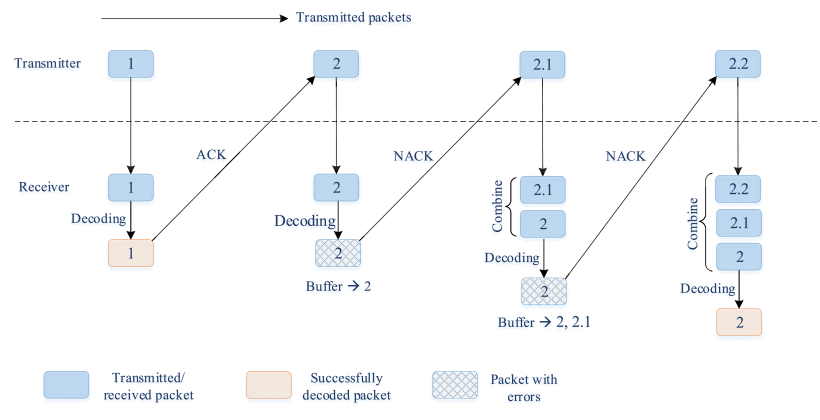
\includegraphics[width=0.9\textwidth]{res/harq-retx-scheme.png}
    \caption{\ac{HARQ} retransmission diagram \cite{harq-wireless-communications-survey}}
    \label{fig:harq_retx_scheme}
\end{figure}

\subsubsection{HARQ working principle}
\paragraph{}
Fig. \ref{fig:harq_retx_scheme} illustrates how \ac{HARQ} processes work. Upon successful reception, depicted in the first column of Fig. \ref{fig:harq_retx_scheme}, an \ac{ACK} is sent back, triggering the transmission of the successive \ac{TB}, which is represented in the second column. This behavior is the normal state in which transmissions are received correctly, and it keeps repeating itself until errors are detected.

\paragraph{} Should the receiver detect errors in the received \ac{TB}, represented by the greyed packet, a \ac{NACK} is sent back to the sender, which in turn proceeds to send some additional redundancy bits. Note that the sender does not repeat the whole \ac{TB}. The receiver now proceeds to decode the transfer block using all the information that it has received so far.

This is the most important feature of \ac{HARQ} protocol: it does not discard the packets affected by errors, since they can be at least used to recover some information. The erroneous packets are stored in buffers and used for joint decoding \cite{5g-nr-harq-devopedia}. 

\paragraph{} If the redundancy bits that the sender just transmitted are still not enough to allow for a correct decoding of the transfer block, or if another error is detected, a retransmission is triggered. This is shown in the last column of Fig. \ref{fig:harq_retx_scheme}. Note that all the information previously received, and not only the last part, is jointly used to decode packet 2.

Finally, if even this retransmission is affected by errors and the combination of the information received so far is not enough to complete the decoding of the \ac{TB}, additional information is sent. After this fourth interaction, no further attempts are made to correct the packet \cite{5g-nr-harq-sharetechnote}.

\paragraph{} The various transmissions and retransmissions being made by the protocol are called \ac{RV}, and are numbered from 0 to 3. Their order can vary depending on the implementation and configuration. Figure \ref{fig:harq_retx_scheme_2} shows another example where the redundancy versions are ordered as 0, 3, 2.

\begin{figure}[ht]
    \centering
    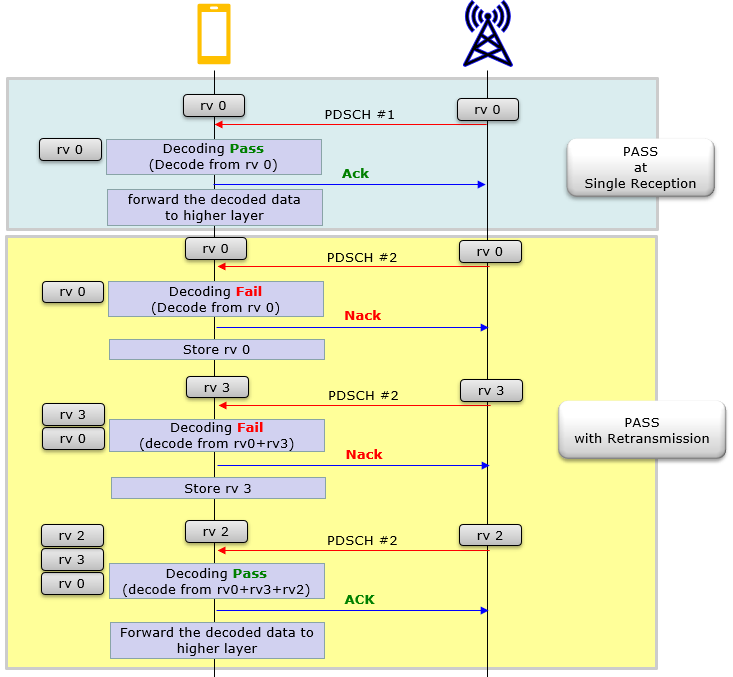
\includegraphics[width=0.9\textwidth]{res/harq-retx-scheme-2.png}
    \caption{\ac{HARQ} diagram with different RVs\cite{5g-nr-harq-sharetechnote}}
    \label{fig:harq_retx_scheme_2}
\end{figure}


\subsubsection{Stop and wait}
\paragraph{} The presented behavior means that \ac{HARQ} is a stop-and-wait kind of protocol, since it is designed to wait for the arrival of previous packet's \ac{ACK} before sending the new one. Figures \ref{fig:harq_retx_scheme_2} and \ref{fig:harq_retx_scheme} highlight this pattern. While this enforces the delivery of ordered packets, it also brings the downside of severely underutilized channel capacity, wasting resources that could potentially be used for transmission instead \cite{3gpp-ts-38.214}. 

This limitation is overcome by the introduction of multiple concurrent processes.

\subsubsection{Processes}
\paragraph{}
A \ac{HARQ} process starts when a \ac{TB} is passed to the \ac{HARQ} entity and finishes when the \ac{ACK} relative to that same \ac{TB} is received by the sender. After the \ac{ACK} is correctly received, the next \ac{TB} starts being processed. Considering a link with propagation delay $\tau_p$, the minimum active time for a process is therefore $2\tau_p$, i.e., the time for the \ac{TB} to arrive to the destination plus the time for the acknowledgement to travel back to the sender.

The 5G \ac{NR} standard allows the base station to configure a certain number of concurrent \ac{HARQ} processes to be assigned to each connected user, ranging from a minimum of 1 (even though the default is 8) to a maximum of 16 \cite{3gpp-ts-38.300, 5g-nr-harq-devopedia}. In this way it is possible to partially limit the effects of the stop-and-wait behavior, allowing for a better throughput.

\subsubsection{Application in NTNs}
\paragraph{}
Since the propagation delay of \ac{NTNs} is orders of magnitude larger than their terrestrial counterpart, the current maximum number of \ac{HARQ} processes, which was optimized for terrestrial transmissions, leads to possible throughput degradation in the NTN domain, as detailed in the following toy example.

\paragraph{Example} Consider a scenario where each process tries to send a \ac{TB} every $2\tau_p$, which is the maximum rate at which transfer blocks can be sent under the condition of waiting for the acknowledgement to arrive before starting a new transmission. The other endpoint is a \ac{LEO} satellite orbiting at 2.000Km, therefore $\tau_p\approx6$ms. Assuming the best possible conditions with no need for retransmissions and assuming 16 concurrent \ac{HARQ} processes, the total send rate is of 16 transfer blocks every 12ms. In order to target a throughput of 50Mbps, the block size must therefore be of at least $$\frac{\textit{target throughput} \times 2\tau_p}{\textit{number of processes}} = 37,5Kb$$
Doing the same calculation for a terrestrial scenario with the \ac{gNB} placed at a distance of 600m from the \ac{UE}, we obtain that the minimum \ac{TBS} must be of just $12b$.
Both calculations do not factor in overheads, control information, channel access requests and processing delays, but are helpful to give an idea of the disproportion in place between the two conditions.

While the necessary block size for the \ac{NTN} case is technically possible to achieve even with the older 4G technology, it necessitates a high \ac{SNR} to work properly. This is because the larger is the block, the higher is the probability of encountering at least one error, therefore more retransmissions would become necessary. This constraint becomes even more conservative in the non-terrestrial case, where the propagation delay is much higher, and retransmissions can quickly become a lot more costly \cite{4g-phy-processing-sharetechnote}.

\section{Possible solutions}
\label{sec:proc-harq-prop-sol}
\subsection{Increasing the number of processes}
The easiest solution would be to increase the number of maximum concurrent \ac{HARQ} processes. Since each process works with a stop-and-wait behavior, the long \ac{RTT} can easily keep all the 16 maximum concurrent processes waiting. While all the processes are waiting their respective \ac{ACK}s, the channel remains unused. Increasing the maximum number of concurrent \ac{HARQ} processes can improve the throughput since the \ac{UE} can spend less time waiting.

However, this comes with some caveats mainly regarding the higher computational capabilities required and higher power consumption, that can quickly become problematic in battery-operated equipment such as smartphones and /or sensors. Each process also requires the presence of a buffer at both the receiver side and the sender side, so additional memory resources are required at the \ac{gNB}, too, which may not be feasible in some application scenarios with strict end user constraints. 
\subsection{Aggressive HARQ}
A more sophisticated approach could involve the design of an aggressive version of the \ac{HARQ} protocol, where each process is allowed to send multiple packets before receiving an acknowledgement e.g., implementing Sliding-Window \ac{HARQ}. Since there already are multiple concurrent processes, each \ac{ACK} packet must already contain a field specifying the number of processes it belongs to, and the information identifying the specific packet to be acknowledged within a process could be encoded inside this field.

\subsection{Disable HARQ}
Lastly, the option of disabling \ac{HARQ} completely and rely solely on \ac{ARQ} retransmissions has been proposed by 3GPP itself \cite{hybrid-arq-schemes-muk}. This, however, would come with a performance penalty in terms of communication accuracy and reliability, since satellite links typically suffer from more severe conditions than terrestrial ones, and \cite{5g-beyond-5g-ntn-trends-vanellicoralli} demonstrated that a version of \ac{HARQ} specifically designed for \ac{NTN}s would be beneficial.

\section{Implemented solution - More processes}
\subsection{Testing current implementation}
\paragraph{}
To test the practical effect that the concurrent \ac{HARQ} processes' limitation has on the achievable throughput, a simulation campaign was conducted where the \ac{HARQ} protocol was firstly disabled and successively enabled, therefore obtaining results for the two different scenarios. The maximum number of concurrent processes with \ac{HARQ} enabled was set to 16, that is the maximum that a \ac{gNB} can allocate to each \ac{UE} according to the 5G \ac{NR} specifications.

\paragraph{}
Comparing the obtained results confirmed that employing \ac{HARQ} caused a noticeable negative impact on the throughput, as illustrated in Fig. \ref{fig:harq_on_off}. The throughput without \ac{HARQ} perfectly matches the source rate, since the \ac{SNR} values of this simulation are high enough to correctly deliver almost the totality of the packets. 

On the other hand, the throughput with \ac{HARQ} enabled reaches its plateau as the source rate crosses the 4Mb/s threshold, settling at this value. \ac{HARQ} struggles to keep up with the increasing source rate since the limited number of processes starts to cause packets to be dropped whenever a retransmission is needed. As the source rate increases, the \ac{HARQ} protocol is completely overwhelmed, as all the 16 processes are always busy, and the arriving packets that do not find an available process are promptly discarded directly at the sender. This is not a retransmission problem, rather a design problem.


\begin{figure}[ht]
    \centering
    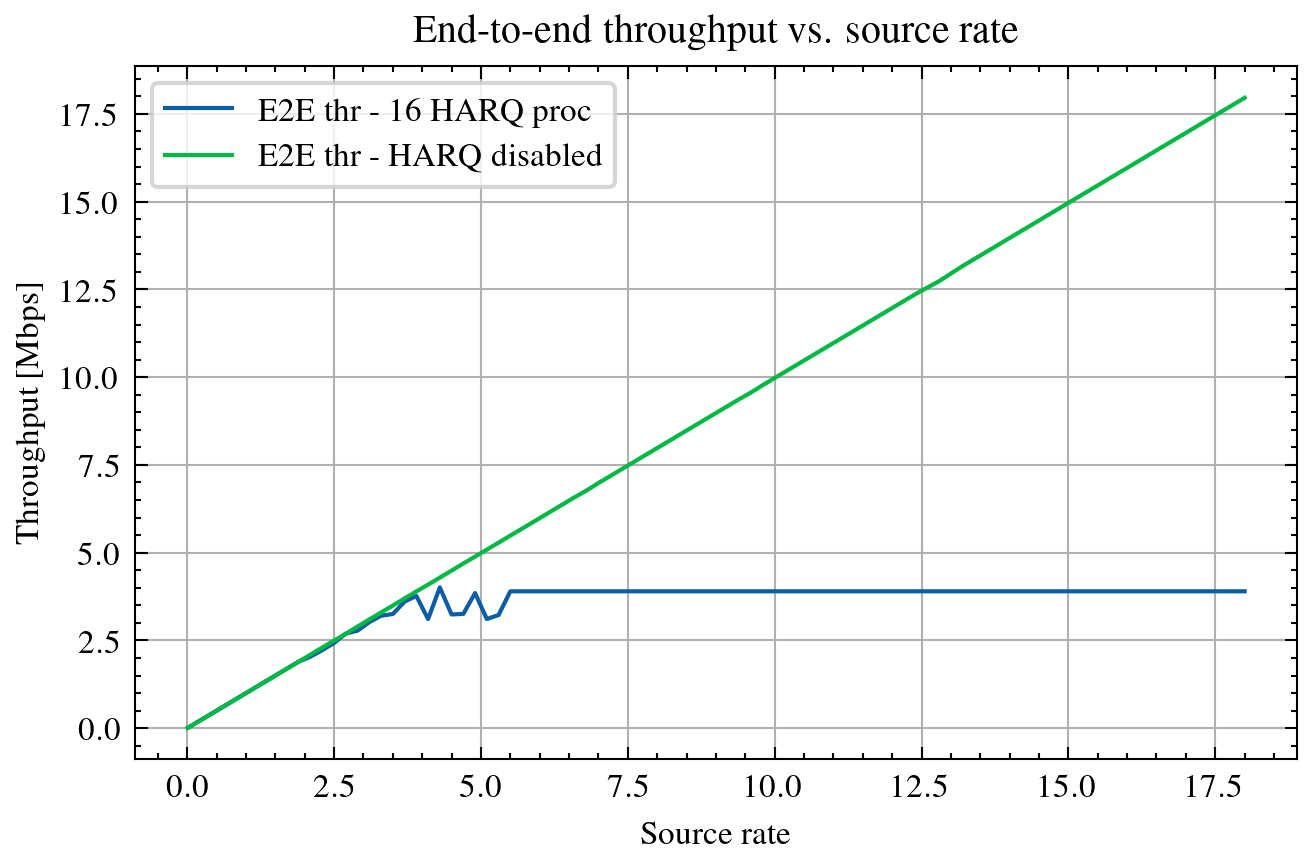
\includegraphics[width=0.8\textwidth]{res/harq-onoff2.png}
    \caption{End-to-end throughput comparison with and without \ac{HARQ}, $\tau_p=6$ms.}
    \label{fig:harq_on_off}
\end{figure}

\begin{figure}[ht]
    \centering
    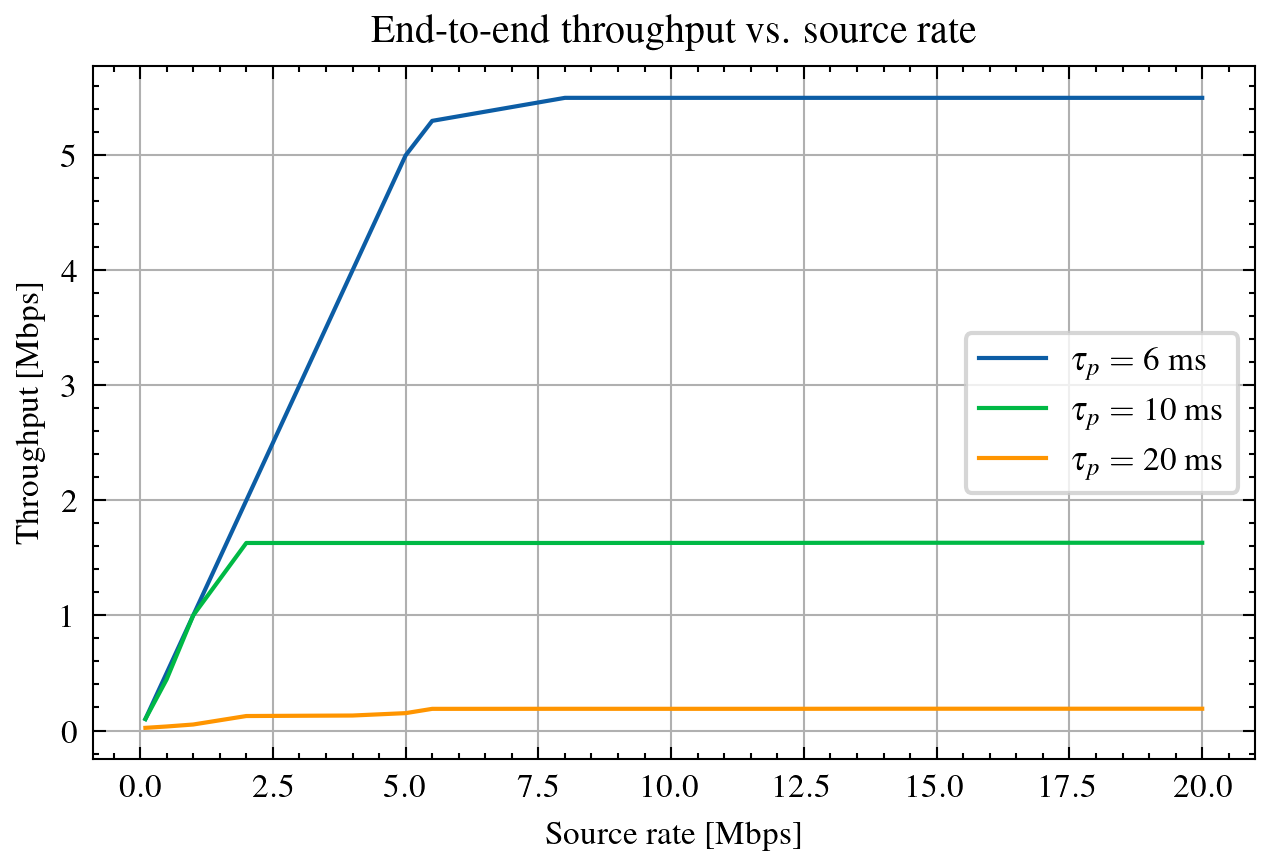
\includegraphics[width=0.8\textwidth]{res/thr_different_tp.png}
    \caption{End-to-end throughput with different propagation delays, 16 \ac{HARQ} processes}
    \label{fig:thr-different-tp}
\end{figure}
\paragraph{Impact of propagation delay}
Figure \ref{fig:thr-different-tp} shows the application-level throughput as the source rate increases, this time while keeping the number of \ac{HARQ} processes fixed to 16 but varying the propagation delay. Simulations were made with $\tau_p\in[20, 40, 60, 80] \text{ms}$. We can see that the maximum achievable throughput is smaller as the propagation delay increases, since each \ac{HARQ} process needs to wait more time for \ac{ACK}s to arrive, dropping newer packets in the meantime.



\subsection{ns-3 implementation}
\paragraph{}
Having verified that \ac{HARQ} does indeed limit the achievable throughput, a modification was implemented to the protocol suite to manually force a higher number of concurrent processes.

This was done by modifying the \texttt{NumHarqProcess} parameter of the class \texttt{MmWavePhyMacCommon}, making it accessible and simulating various scenarios with different number of processes.

However, a flaw in the \texttt{MmWaveFlexTtiMacScheduler} class in the ns-3 implementation of \ac{HARQ} made the whole simulator crash whenever a new outbound packet found that all the processes were already occupied. If $n$ processes were available, the simulator tried to access the $n+1$th process, causing an exception. The implemented solution consisted of a safeguard that checked the number of available processes, eventually discarding the packet. 


\begin{figure}[ht]
    \centering
    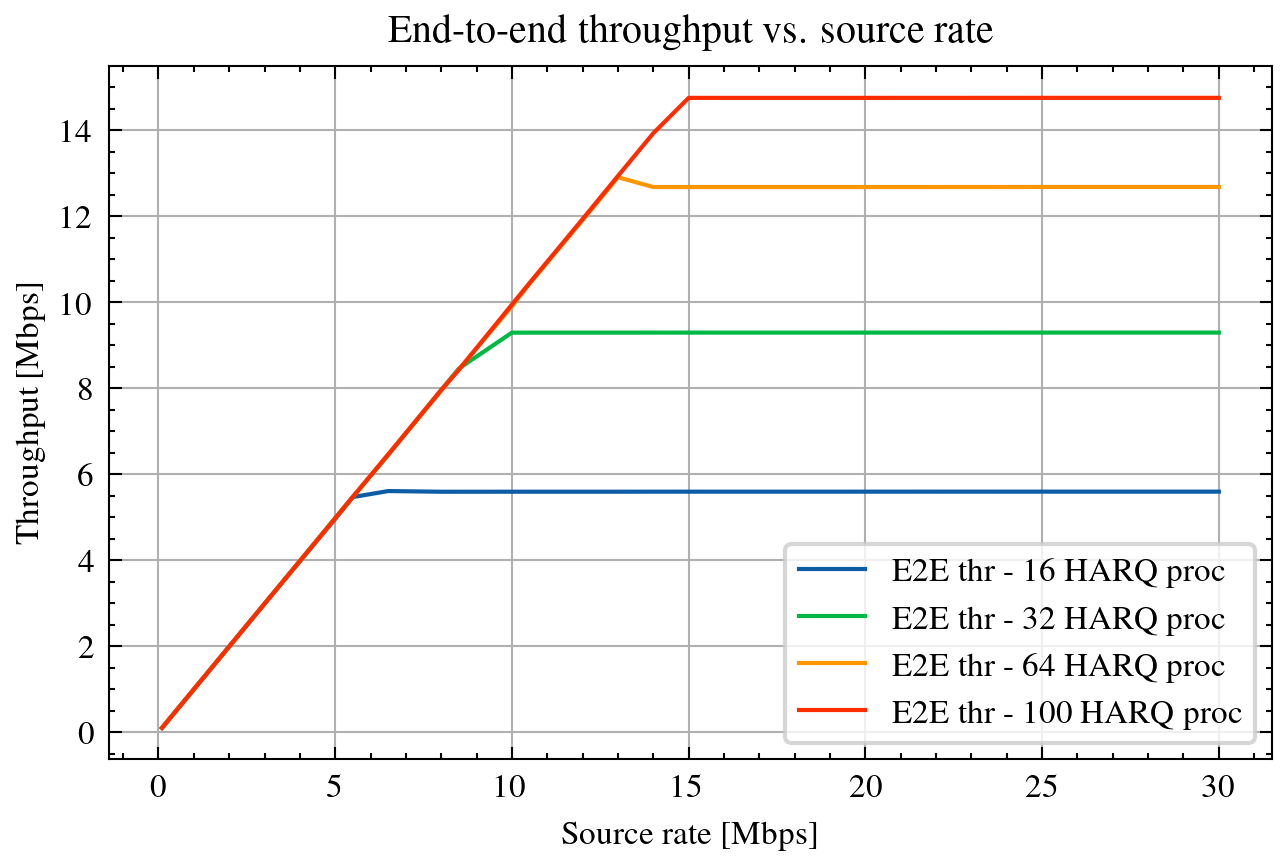
\includegraphics[width=0.8\textwidth]{res/thr_processes.png}
    \caption{End-to-end throughput comparison with different number of concurrent \ac{HARQ} processes, $\tau_p=6$ms.}
    \label{fig:harq-numproc}
\end{figure}

\subsection{Results}
\paragraph{}
The results shown in figure \ref{fig:harq-numproc} make clear that increasing the parameter regulating the number of \ac{HARQ} processes allows for higher throughput. Each line in the plot was obtained with a different number of allowed processes, starting from 16, the maximum possible value in the 5G \ac{NR} standard, then 32, 64 and ultimately 100. No further increases have been evaluated, since those would currently be unrealistic to achieve.

Increasing the allowed number of \ac{HARQ} processes pushed the maximum achievable throughput up to around 14 Mb/s when considering 100 parallel processes. Going past such threshold causes packets to start being dropped, and the throughput to saturate, since there are no more available processes to send the traffic generated by the application.

However, constraints regarding the required computational power and the increased energy and memory consumption shall also be taken into careful consideration, since raising the number of concurrent processes from 16 to 100 is a big step, bringing a consistent increase in both the receiver and transmitter complexity with it.

We can conclude that, while certainly being a way to improve the performances of \ac{HARQ} in non-terrestrial scenarios, the increase in processes alone cannot solve the problem of \ac{HARQ} limiting the throughput, therefore other ways have to be found, and future studies should also consider alternative proposals.


\section{Implemented solution - Disabling HARQ}
\paragraph{}
Figure \ref{fig:harq_on_off} could suggest that completely disabling the \ac{HARQ} protocol could be a viable solution, since the end to end throughput of the simulation with \ac{HARQ} switched off always matched the source rate, meaning that all the packets generated by the application were correctly received by the remote host.

However, the reason of this behavior is the high \ac{SNR} that was forced in the simulated scenario with the choice of using high gain antennas. This design choice is not fully realistic, espcially considering direct-to-handle communication. Such choice was made because this thesis is focused on the study of the propagation delay, and the high gain of aperture antennas allowed to limit the impact of some other problems caused by low \ac{SNR}. Having a communication channel with high \ac{SNR} allowed for fewer variables to impact the simulations' results, in turn enabling the study of propagation delay alone.

\paragraph{}
In order to test the performances without \ac{HARQ} enabled, a new simulation campaign was conducted factoring in the problems related to poor \ac{SNR}, such as the presence of errors in the received packets and the need for retransmissions. The gain of the \ac{UE}'s antenna was lowered in order to appreciate the difference between the case with \ac{HARQ} enabled and the case with \ac{HARQ} disabled. In conditions of low \ac{SNR}, e.g., when the distance between the terrestial end node and the satellite (and so the propagation delay) increases, which can be plausible in a non-terrestrial communication scenario, the \ac{PDR} and therefore the throughput can drop considerably, impacting the link reliability.

\begin{figure}[ht]
    \centering
    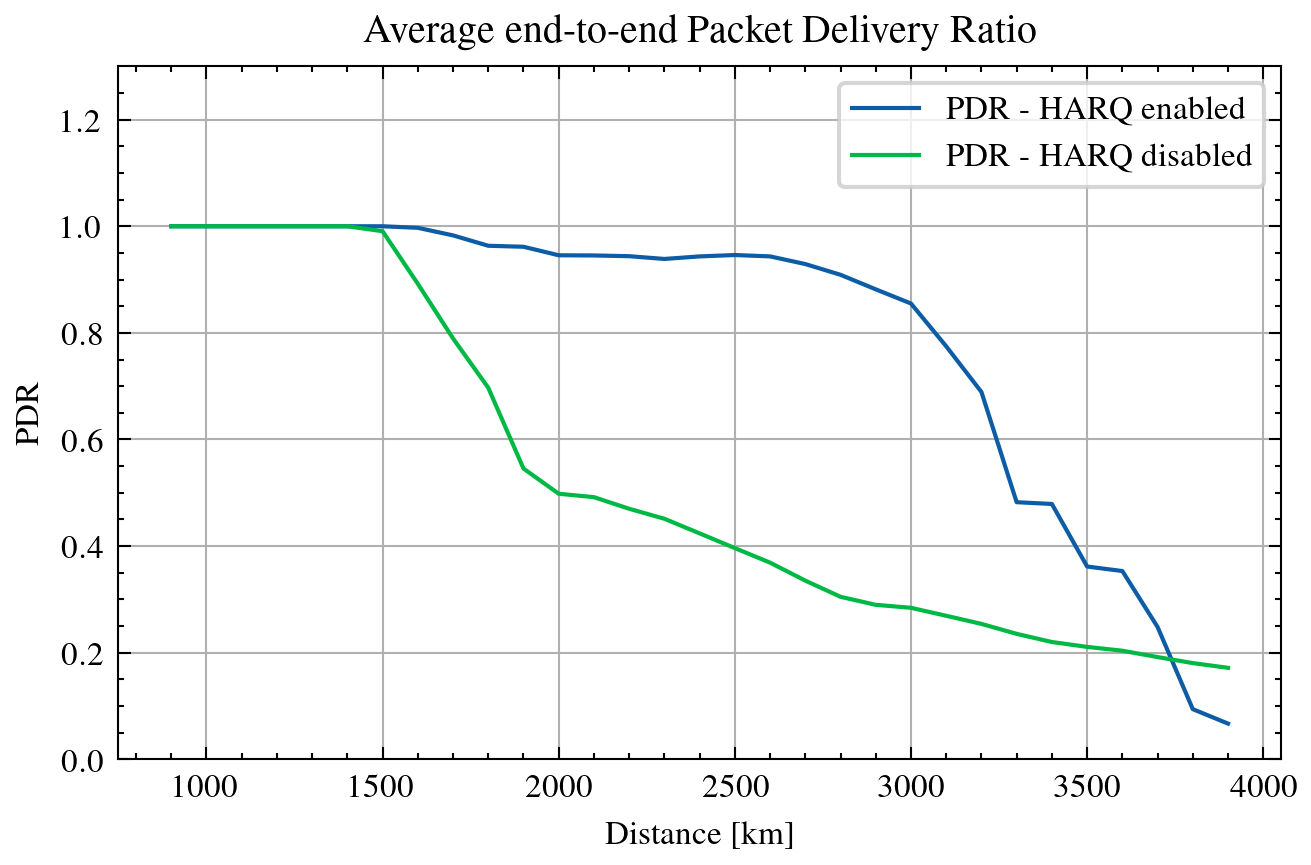
\includegraphics[width=0.8\textwidth]{res/pdr_harq_onoff.png}
    \caption{Packet delivery ratio with \ac{HARQ} on and off, 16 concurrent \ac{HARQ} processes}
    \label{fig:harq-snr}
\end{figure}

\paragraph{}
Simulations have shown that disabling \ac{HARQ} is a good solution only when both \ac{UE} and \ac{gNB} experience good channel conditions with high \ac{SNR}, while poor channel conditions benefit from having \ac{HARQ} enabled. Figure \ref{fig:harq-snr} shows the packet delivery ratio as the orbiting altitude of the satellite increases, thus reducing the SNR. Initially, both scenarios correctly deliver all the packets, but, as the link quality decreases, the use of \ac{HARQ} protocol proves to be beneficial for the reliability of the transmission, since it manages to correctly deliver more packets. 

A hybrid approach can also be thought, where \ac{CQI} can be used to assess the state of the channel and decide whether to enable \ac{HARQ}, therefore limiting the throughput in exchange for a higher reliability, or disabling it, should the \ac{SNR} be high enough.

\section{Implemented solution - Aggressive HARQ}
\paragraph{}
In the previous section we disabled \ac{HARQ} and compared the link reliability against the same scenario with \ac{HARQ} enabled. Results showed that \ac{HARQ} is still beneficial in cases of low \ac{SNR}, therefore a modification was designed and implemented to try optimizing the protocol's behavior when dealing with high propagation delays.
Now each \ac{HARQ} process is allowed to send two packets at once without having to wait for the \ac{ACK} to arrive. Once the \ac{ACK} arrives, the process can send two more packets and so on.

\begin{figure}[ht]
    \centering
    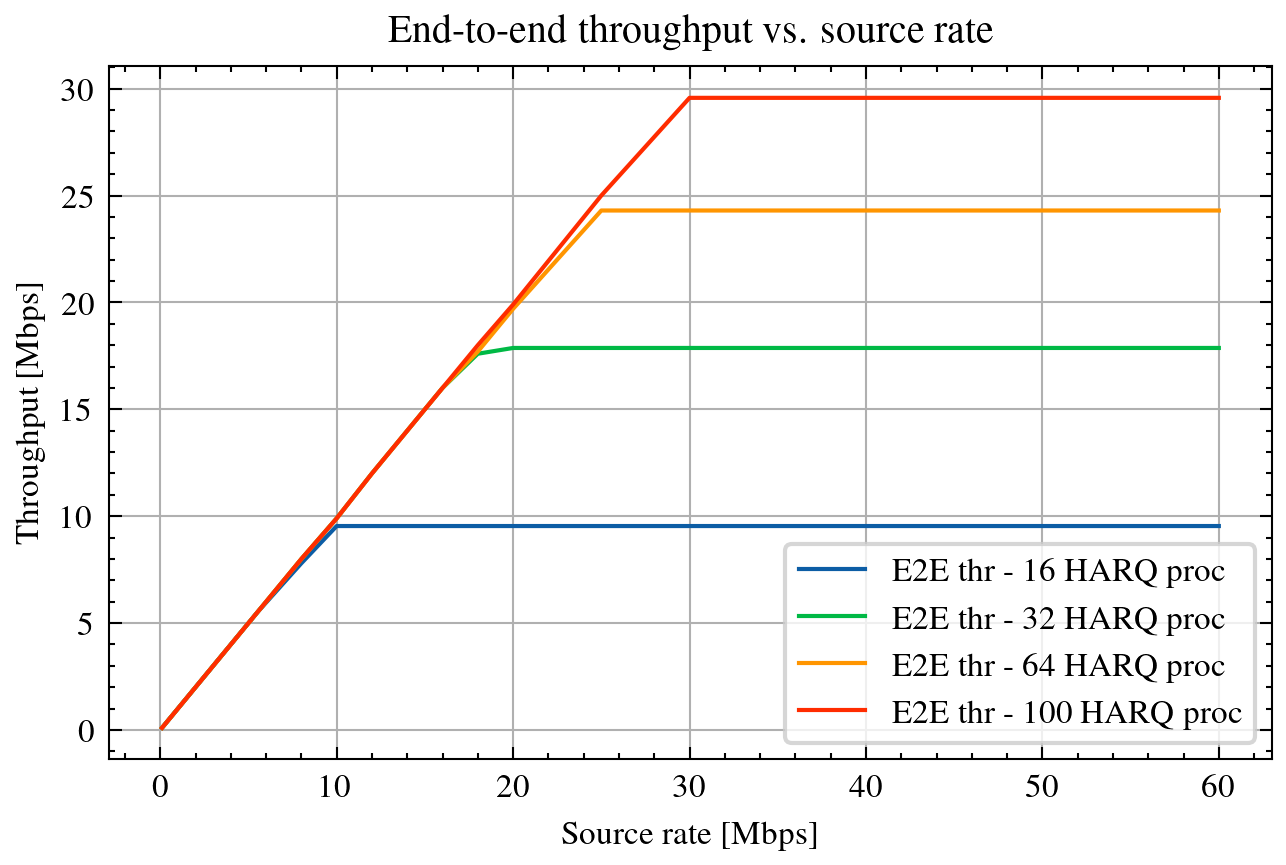
\includegraphics[width=0.8\textwidth]{res/aggressive_harq.png}
    \caption{End-to-end throughput comparison with aggressive \ac{HARQ}.}
    \label{fig:aggressive}
\end{figure}

\paragraph{}
Figure \ref{fig:aggressive} shows the results of the aggressive \ac{HARQ} approach. Each line in the plot represents a different number of maximum concurrent \ac{HARQ} processes allocated to each user. 

As expected, for each number of concurrent \ac{HARQ} processes, the throughput is roughly doubled with respect to the standard \ac{HARQ} implementation of Figure \ref{fig:harq-numproc}, while the overall trend is similar.

\paragraph{Drawbacks}
This approach could be further pushed to accomodate for even more packets per process, allowing for a higher throughput to be achieved. However, we expect to incur in a penalty in terms of additional overheads caused by both control messages and packets retransmissions. Furthermore, additional resources are required, both in terms of computational capabilities and memory. 

\iffalse
    \subsection{Simulator configuration}
    While the number of concurrent HARQ processes can be configured in ns-3, it cannot exceed the value of 100. By performing some simple calculations, knowing that the \ac{SNR} conditions allow for the transmissions of \ac{TB}s with size of 1024B, to achieve a target throughput of 50Mbps on the best case of 6ms $\tau_p$ the necessary processes would be 74.
    $$\frac{\textit{target throughput} \times 2\tau_p}{\textit{total block size}} \approx 74 \textit{processes}$$

    This does not account for the delays caused by retransmissions, so simulator crashes due to processes overflow are frequent while testing even the best case scenario.

\fi


    %!TEX root = ../main.tex

\chapter{Conclusions and Future Works}
\label{chp:conclusions}

This work has provided a comprehensive study on the impact that the high propagation delay experienced in \ac{NTN}s has in layer-2 protocols. The current codebase of the ns-3 network simulator has been properly extended to allow for end-to-end simulation of the \ac{NR} stack in a \ac{NTN} scenario, since the ns-3 implementation of \ac{NR} technology was not designed for high propagation delays. A lot of work went therefore into the design, implementation, and testing of a base support for the simulation of \ac{NTN}s.

It was shown that propagation delay plays a crucial role in the performances of \ac{NR} in \ac{NTN}s, affecting both the efficiency and reliability of data transmission.

\paragraph{}
Once the simulator was ready, focus has been placed on the optimization of the \ac{HARQ} protocol in \ac{NTN}s, investigating its shortcomings when delaing with large propagation delays as well as proposing some original solutions to increase its performances.

\section{Results}
\subsection{Simulator redesign}
Since the state of the art in network simulation tools was not ready for complete \ac{NR} \ac{NTN} simulations, presenting numerous problems especially at the scheduler, a redesign of certain behaviors was performed.

\subsubsection{Scheduling with propagation delay}
This study has found (section \ref{sec:pd-sched-acc}) that the current scheduling with short advance (i.e. scheduling only a slot in advance: at time $t_0$ the schedule allocates the resources of time $t_0+1$ms) does not work in \ac{NTN} because the propagation delay itself is longer than the delay between the act of scheduling and the time for which the scheduling happens. 

The proposed solution uses information on the propagation delay to adjust the advance of the scheduling process. 

\subsubsection{BSR timer}

Another flaw discovered in the implementation of current \ac{NR} protocols in \ac{NTN} involves the periodic \ac{BSR} that the \ac{UE} keeps sending every 10ms (section \ref{sec:bsr-timer}). 

While this approach presents some (undesired) benefits, it is not the intended behavior, therefore the current implementation, albeit working, is far from an ideal choice.

The proposed solution consists of adapting the \ac{BSR} timer accordingly to the propagation delay, never allowing it to assume values smaller than a round-trip time. 

\subsubsection{Inflated BSR}
If the interval between the packets generated by the application is smaller than the \ac{RTT}, each \ac{BSR} will report the whole size of the transmission buffer, even though other \ac{SR} relative to packets already present in the buffer may be still in-flight. While leading to an overall lower latency, this vastly increases the amount of resources being wasted, since the \ac{UE} will find itself with many unnecessary transmission grants (Section \ref{sec:inf-bsr}).

The proposed solution is to limit the scheduling requests that are triggered every time a packet arrives into the transmission buffer to the new data only.

\subsubsection{Reordering timer}
The conducted simulation campaigns have found that anytime a packet is fragmented and sent across multiple frames, a reordering and recomposition timer is activated at the \ac{gNB} side, which, however, is too short with respect to the large propagation delay in \ac{NTN}s, expiring before all the pieces of the packet have the chance to arrive (Section \ref{sec:reord-timer}).

The implemented solution was to extend such timer in order to account for the propagation delay.

\subsection{HARQ}
\subsubsection{Concurrent processes}
This work confirmed that the 16 maximum concurrent \ac{HARQ} processes allowed per user heavily limits the achievable throughput (section \ref{sec:harq-conc-proc}).

Different solutions have been proposed, including completely disabling the protocol as well as increasing the number of allowed concurrent processes.

Both these solutions have also been implemented in the simulator, evaluating scenarios with no \ac{HARQ}, then 16, 32, 64 and 100 maximum concurrent processes. 

It was found that increasing the number of processes allows for considerably higher throughputs, while disabling \ac{HARQ} is only feasible in conditions of high \ac{SNR}.

Since having \ac{HARQ} enabled still proved to be helpful in a scenario of low \ac{SNR}, a more aggressive version of \ac{HARQ} was designed, where each process was allowed to send two packets instead of one before waiting for the \ac{ACK}. This solution managed to roughly double the achievable throughput with respect to the standard \ac{HARQ} implementation.

\section{Future work}

The preparation of this work required many simulations to be run and evaluated, and as expected some design problems emerged. With a thoughtful approach, each unexpected behavior was investigated and solutions were devised, implemented and tested.

While effort was made to provide more than a single solution, striving to look at the problems from different perspectives to find more than a single way to approach it, some possibilities still require a deeper study, and some observations were made whenever it was felt that a point might benefit from additional work.

This section describes some possible future paths that might have the potential to improve the solutions proposed in this work, as well as different approaches which performances are still to be evaluated.

\paragraph{}
The current behavior of waiting for packets to arrive at the transmission buffer of the \ac{UE} before transmitting the \ac{SR} to the \ac{gNB} harshly impacts the experienced latency, since in the best-case scenario it at least adds a round-trip time of delay. While this is not a problem in terrestrial networks because base stations are relatively close to the \ac{UE}s that are serving, in \ac{NTN}s the added delay is noticeable. 

A predictive algorithm capable of visualizing patterns in the \ac{UE}-generated traffic, forecasting its behavior in the immediate future and preemptively sending \ac{SR} so that new packets will be able to be transmitted right away without additional delays would be of invaluable help in reducing the overall latency of the link.

\paragraph{}
Timers often represent a trade-off between higher performances and a more robust network. This is the reason behind the proposal of a dynamic approach when setting the values for \ac{BSR} periodic requests and reordering timer. Since the delay of \ac{NTN}s can experience large variations depending on the satellite orbit, configurable timers shall be preferred instead of using fixed values.

\paragraph{}
Regarding \ac{HARQ}, a dynamic way of enabling and disabling it on the fly based on channel quality indicators could be beneficial, since it was shown that high-\ac{SNR} scenarios performed better with \ac{HARQ} disabled, while conditions of low \ac{SNR} benefitted from having it enabled.

\paragraph{}

It is clear that further research is needed to develop more effective strategies for managing propagation delay in \ac{NTN}s. This includes exploring new technologies, improving existing methodologies, and devising innovative network architectures.

Ultimately, this work aims to pave the way for future research and practical applications in the field of \ac{NTN}s, emphasizing the need for continuous innovation and adaptation to meet the evolving demands of modern communication systems. 

The findings of this thesis not only contribute to the existing body of knowledge on \ac{NTN}s but also pave the way for future research in this evolving field.

    
    % Bibliography, appendix, acknowledges, etc...
    \backmatter
\end{document}